\documentclass[12pt,a4paper,titlepage,listof=totoc,bibliography=totoc,chapteratlists=0pt]{scrreprt}

\begin{filecontents*}{\jobname.xmpdata}
	\Keywords{VR, IOT, TODO}
	\Title{Unser tolles Thema -- wir sind suppa}
	\Author{Stefan Schwammal, Susi Schwammal}
\end{filecontents*}

\setcounter{tocdepth}{1}

\usepackage[utf8]{inputenc}
\usepackage[T1]{fontenc}
\usepackage{amsmath}
\usepackage{amsfonts}
\usepackage{amssymb}
\usepackage[table]{xcolor}
\usepackage{graphicx}
\usepackage[left=3.50cm, right=2.00cm, top=2.00cm, bottom=2.00cm,foot=1cm]{geometry}
\usepackage[splitrule,hang,flushmargin,multiple,bottom]{footmisc}
\usepackage{lmodern, textcomp}
\usepackage{lmodern}
\usepackage{pdfpages}
\usepackage[ngerman]{babel}
\usepackage{multicol}
\usepackage{subfig}
\usepackage{float}
\usepackage{array,tabularx,booktabs}
\usepackage{ragged2e}
\usepackage{lipsum}
\usepackage{wrapfig}

\newcolumntype{M}[1]{>{\centering\arraybackslash}m{#1}}

\usepackage{enumitem}
\newlist{compactitem}{itemize}{3}
\setlist[compactitem,1]{label=\textbullet, nosep,leftmargin=1.5em,labelwidth=*,align=left}
\setlist[compactitem,2]{label=--, nosep,leftmargin=1.5em,labelwidth=*,align=left}
\setlist[compactitem,3]{label=\textopenbullet, nosep,leftmargin=1.5em,labelwidth=*,align=left}
\newlist{compactenum}{enumerate}{3}
\setlist[compactenum,1]{label=\arabic*., nosep,leftmargin=1.5em,labelwidth=*,align=left}
\setlist[compactenum,2]{label=\alph*., nosep,leftmargin=1.5em,labelwidth=*,align=left}
\setlist[compactenum,3]{label=\roman*., nosep,leftmargin=1.5em,labelwidth=*,align=left}
\newlist{compactdesc}{description}{3}
\setlist[compactdesc]{leftmargin=1.5em,labelwidth=*,align=left}

\usepackage{microtype}

\usepackage[parfill]{parskip}

\definecolor{bluekeywords}{rgb}{0.13,0.13,1}
\definecolor{greencomments}{rgb}{0,0.5,0}
\definecolor{redstrings}{rgb}{0.9,0,0}
\definecolor{lightgray}{gray}{0.9}
\definecolor{lightblue}{rgb}{0.93,0.95,1.0}

\usepackage{listings}

\makeatletter
\lstdefinestyle{lststyle}{
	basicstyle=%
	\ttfamily
	\lst@ifdisplaystyle\scriptsize\fi
}
\makeatother

\renewcommand{\lstlistlistingname}{List of Listings}
% TODO: define other languages as needed
\lstset{language=Python,
numbers=left,               
numberstyle=\tiny,          
showspaces=false,
showtabs=false,
breaklines=true,
lineskip=-1pt,
tabsize=2,
showstringspaces=false,
breakatwhitespace=true,
escapeinside={(*@}{@*)},
commentstyle=\color{greencomments},
keywordstyle=\color{bluekeywords}\bfseries,
stringstyle=\color{redstrings},
style=lststyle,
xleftmargin=17pt,
         framexleftmargin=17pt,
         framexrightmargin=5pt,
         framexbottommargin=4pt
}
\lstset{
morekeywords={base,var,in,out,dynamic,from,where,select,orderby,function,\$,group,by,into,yield,async,await,@,None,self,as,elif,with}
}
\lstdefinelanguage{TypeScript}{
	keywords={typeof, new, true, false, catch, function, return, null, switch, var, if, in, while, do, else, case, break, void, number, string, boolean, module, \$, export, for, this},
	keywordstyle=\color{blue}\bfseries,
	ndkeywords={class, export, boolean, throw, implements, import, this},
	ndkeywordstyle=\color{darkgray}\bfseries,
	identifierstyle=\color{black},
	sensitive=false,
	comment=[l]{//},
	morecomment=[s]{/*}{*/},
	commentstyle=\color{purple}\ttfamily,
	stringstyle=\color{red}\ttfamily,
	morestring=[b]',
	morestring=[b]"
}
\usepackage{caption}
\DeclareCaptionFont{white}{\color{white}}
\DeclareCaptionFormat{listing}{\colorbox[cmyk]{0.43, 0.35, 0.35,0.01}{\parbox{\textwidth}{\hspace{10pt}#1#2#3}}}
\captionsetup[lstlisting]{format=listing,labelfont=white,textfont=white} 
\captionsetup[table]{justification=centering, singlelinecheck=false}

\usepackage{setspace}
\newcommand{\MSonehalfspacing}{%
	\setstretch{1.44}%  default
	\ifcase \@ptsize \relax % 10pt
	\setstretch {1.448}%
	\or % 11pt
	\setstretch {1.399}%
	\or % 12pt
	\setstretch {1.433}%
	\fi
}

\newcommand{\setauthor}[1]{\ohead[]{#1}}

\usepackage[automark]{scrlayer-scrpage}
\pagestyle{scrheadings}
\automark{chapter}
\renewcommand\sectionmark[1]{\markright{\MakeMarkcase {\thesection\hskip .5em\relax#1}}}
\rohead{\ifnum\expandafter\pdfstrcmp\botmark=0 \rightmark\else\leftmark{} --- \rightmark\fi}
\ihead[]{\headmark}
\chead[]{}
\ohead{}
\cfoot[]{}
\ofoot[\pagemark]{\pagemark}
\setheadsepline{.1pt}

\usepackage[hyphens]{url}

\usepackage[a-1b]{pdfx}

\usepackage{hyperref}
\hypersetup{pdfa}

\usepackage[nonumberlist,toc,nopostdot]{glossaries}

\usepackage{chngcntr}
\counterwithout{footnote}{chapter}
\counterwithout{figure}{chapter}
\counterwithout{table}{chapter}
\AtBeginDocument{
	\counterwithout{lstlisting}{chapter}
	\urlstyle{sf}
}
\newcounter{RPages}

\makeatletter
\def\bstctlcite{\@ifnextchar[{\@bstctlcite}{\@bstctlcite[@auxout]}}
\def\@bstctlcite[#1]#2{\@bsphack
	\@for\@citeb:=#2\do{%
		\edef\@citeb{\expandafter\@firstofone\@citeb}%
		\if@filesw\immediate\write\csname #1\endcsname{\string\citation{\@citeb}}\fi}%
	\@esphack}
\makeatother

\clubpenalty=10000
\widowpenalty=10000
\displaywidowpenalty=10000
\interfootnotelinepenalty=10000

\title{Beam VR -- Synchronized Realities}
\author{Quirin Ecker, Florian Beckerle}

\makeindex
\makeglossaries
\begin{document}
\bstctlcite{IEEEexample:BSTcontrol}
\newcommand{\reminder}[1]
{ \textcolor{red}{<[{\bf\marginpar{\mbox{$<==$}} #1 }]>} }
\newcommand{\icode}[1]{\lstinline$#1$}
%\urlstyle{same}
%\setstretch{1.5}
\setstretch {1.433}
\renewcommand{\arraystretch}{1.2}

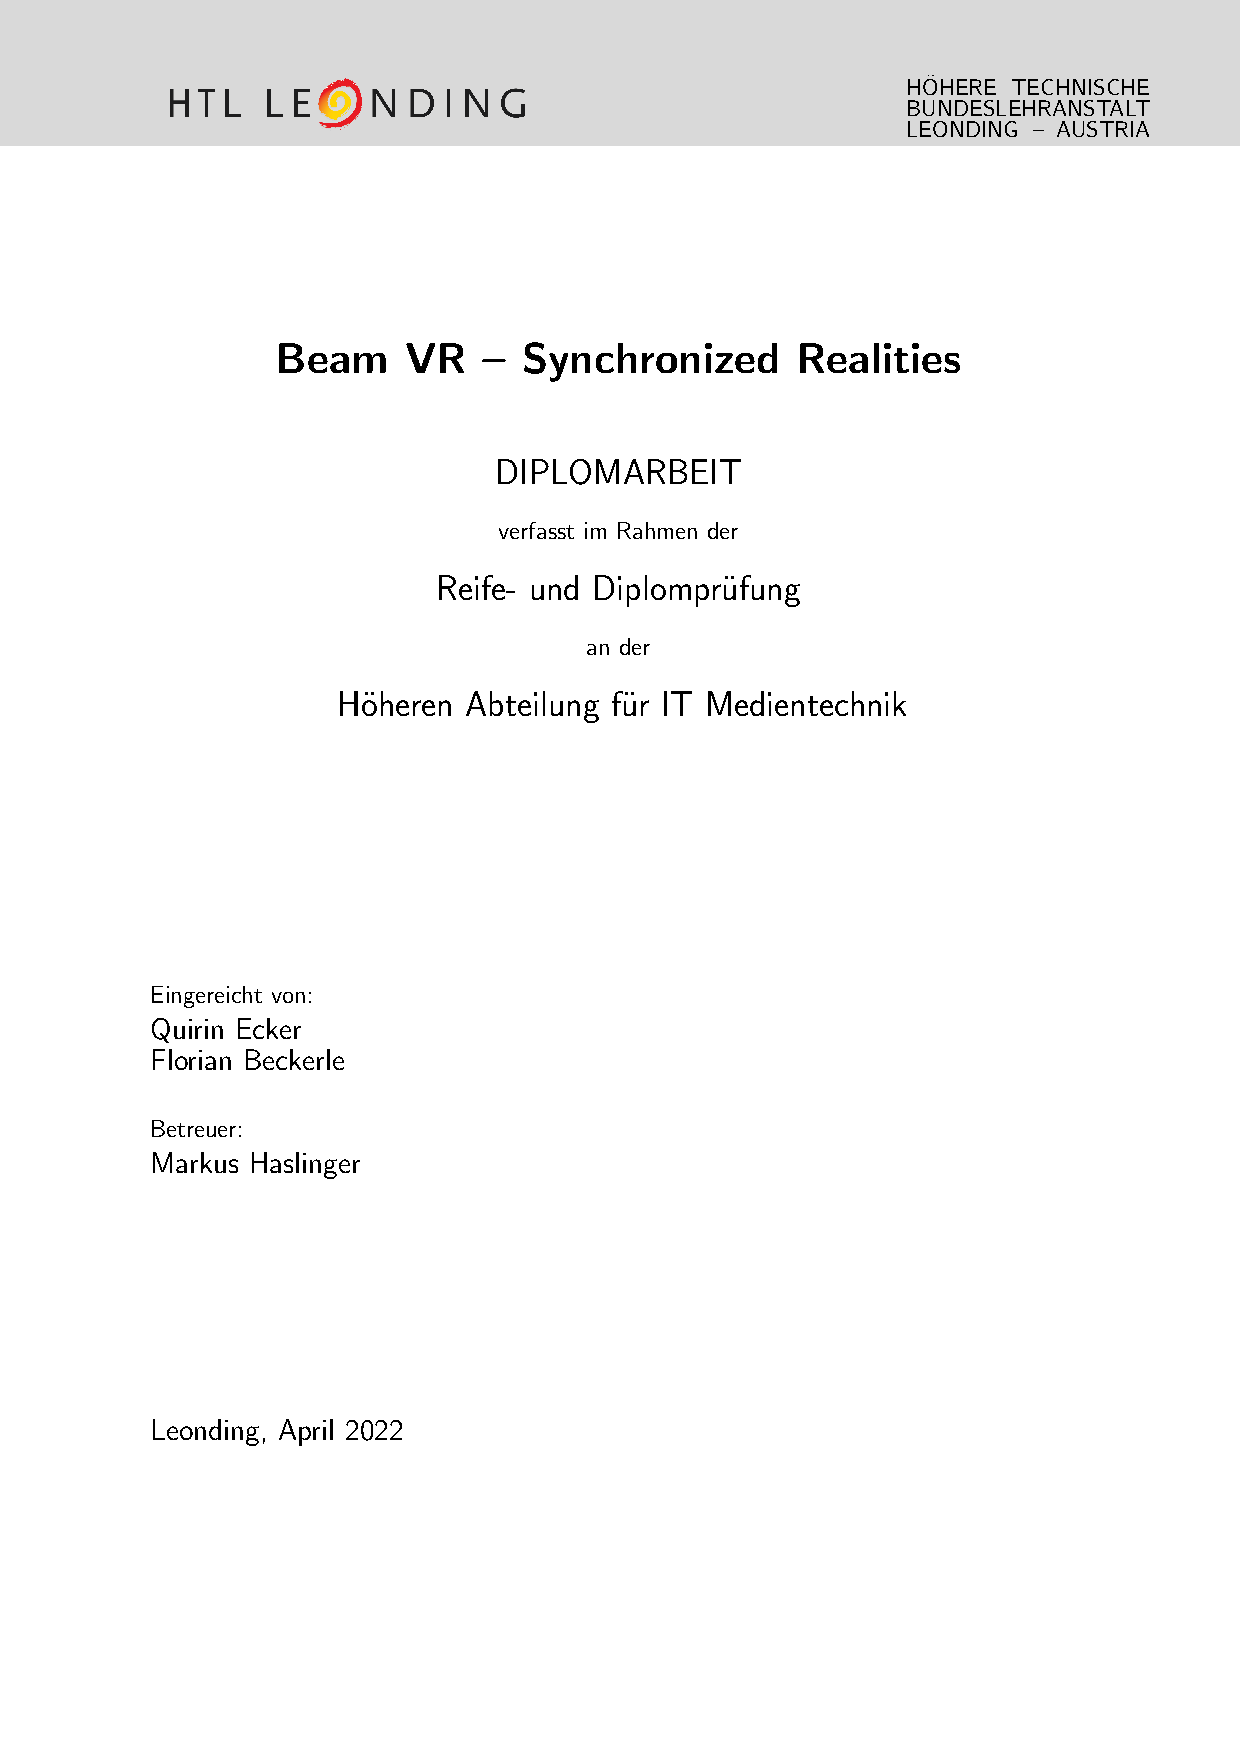
\includepdf{./titlepage/coversheet}
\pagenumbering{Roman}
\newpage
\thispagestyle{empty}
\vspace{3cm}
~ \\ \\
Ich erkläre an Eides statt, dass ich die vorliegende Diplomarbeit selbstständig und ohne fremde Hilfe verfasst, andere als die angegebenen Quellen und Hilfsmittel nicht benutzt bzw. die wörtlich oder sinngemäß entnommenen Stellen als solche kenntlich gemacht habe.

Die Arbeit wurde bisher in gleicher oder ähnlicher Weise keiner anderen Prüfungsbehörde vorgelegt und auch noch nicht veröffentlicht.

Die vorliegende Diplomarbeit ist mit dem elektronisch übermittelten Textdokument identisch.
\vspace{3cm}
% Hier kommt die Unterschrift drüber
\begin{tabbing}
Leonding, April 2022 \hspace{5cm} S. Schwammal \& S. Schwammal
\end{tabbing}
\vspace{10cm}
Zur Verbesserung der Lesbarkeit wurde in diesem Dokument auf eine geschlechtsneutrale Ausdrucksweise verzichtet.
Alle verwendeten Formulierungen richten sich jedoch an beide Geschlechter.
\newpage
\setcounter{page}{1}
\begin{spacing}{1}

    \chapter*{Abstract}

\end{spacing}

\begin{wrapfigure}{r}{0.3\textwidth}

    \begin{center}

        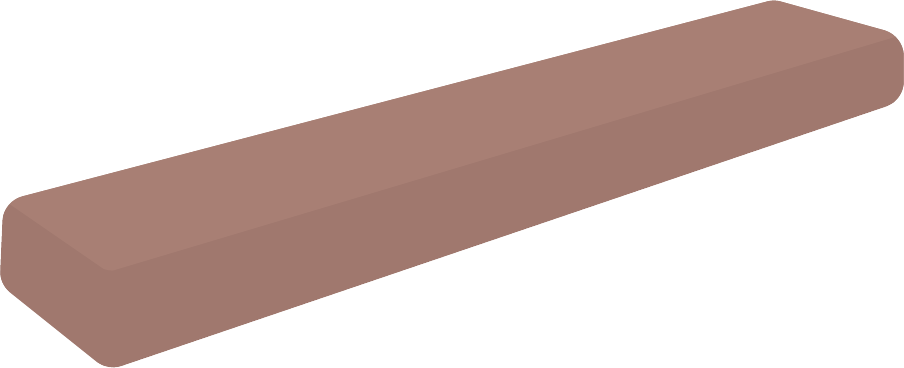
\includegraphics[width=0.2\textwidth]{pics/abstract_picture_1}

    \end{center}

\end{wrapfigure}

Beam VR is a project which aims to give an immersive experience of height.
It consists of a scene on top of a building with a plank, which protrudes from this building.
To increase the immersion we use virtual reality combined with the physical reality (Augmented Virtuality).
In particular the plank exists in the virtual as well as in the physical reality.

With a realistic environment including cars, high skyscrapers and classic new york city sounds we optimize the immersion of the reality.
The objective of the simulation is balancing on the beam without falling off.
Furthermore, the scene can be experienced in three different maps, namely Night, Day and Apocalypse.

\newpage

\begin{spacing}{1}

    \chapter*{Zusammenfassung}

\end{spacing}

\begin{wrapfigure}{r}{0.3\textwidth}

    \begin{center}

        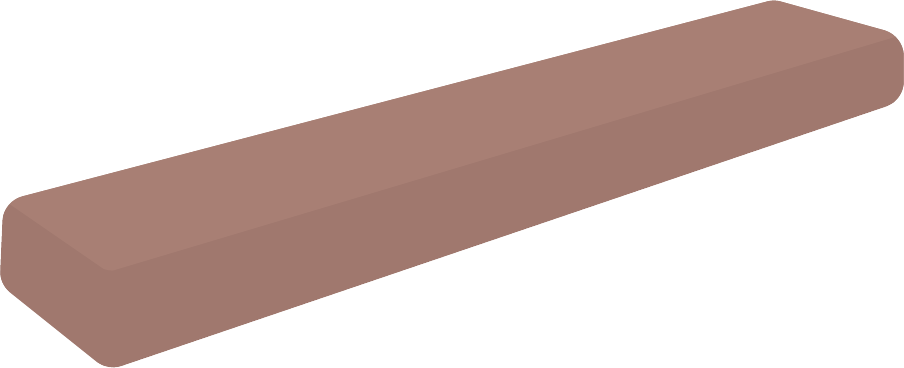
\includegraphics[width=0.2\textwidth]{pics/abstract_picture_1}

    \end{center}

\end{wrapfigure}

Beam VR ist ein Projekt, das darauf abzielt, ein immersives Höhenerlebnis zu vermitteln.
Es besteht aus einer Szene auf einem Gebäude mit einem Brett, das aus diesem Gebäude herausragt.
Um die Immersion zu steigern, verwenden wir Virtual Reality in Kombination mit der physischen Realität (Augmented Virtuality).
Insbesondere das Brett existiert sowohl in der virtuellen als auch in der physischen Realität.

Mit einer realistischen Umgebung aus Autos, hohen Wolkenkratzern und klassischen New-York-City-Sounds optimieren wir das Eintauchen in die Realität.
Ziel der Simulation ist es, auf dem Balken zu balancieren, ohne herunterzufallen.
Darüber hinaus kann die Szene in drei verschiedenen Karten erlebt werden, nämlich Night, Day und Apocalypse.

\begin{spacing}{1}

    \chapter*{Danksagung}

\end{spacing}

An dieser Stelle möchten wir uns bei all jenen bedanken, die durch ihre fachliche, persönliche und finanzielle Unterstützung zum Gelingen dieser Diplomarbeit beigetragen haben.

Besonders möchten wir uns bei Pärtel Lang bedanken, welcher uns netterweise das FinalIK Plugin für diese Arbeit zur Verfügung gestellt hat.

Außerdem sind wir dem Unternehmen Nimbuscloud sehr dankbar, da diese ein Büro zur Bearbeitung unserer Diplomarbeit zur Verfügung gestellt haben.

Schlussendlich möchten wir uns noch bei unserem Betreuer Herr Professor Haslinger und bei dem Abteilungsvorstand Peter Bauer für die fachliche und persönliche Unterstützung während der Implementierung bedanken.


\pagestyle{plain}

\renewcommand{\lstlistlistingname}{Quellcodeverzeichnis}

\setcounter{tocdepth}{2}
\tableofcontents
\newpage
\setcounter{RPages}{\value{page}}
\setcounter{page}{0}
\pagenumbering{arabic}
\pagestyle{scrheadings}

\begin{spacing}{1}
\chapter{Einleitung}\label{chapter:introduction}
\end{spacing}
\section{Ausgangssituation}\label{sec: initial_situation}

Es gibt bereits viele VR Applikation, aber was ist genau eine VR Applikation.
Es gibt viele Definitionen für VR ausgeschrieben Virtual Reality.
In dieser Arbeit sprechen wir über die Wirklichkeit welche durch ein head mounted display, oder umgangssprachlich auch eine VR-Brille angezeigt wird.
Somit bezeichnet eine VR Application eine Software, welche in der VR-Brille läuft.

Von diesen VR Applikationen gibt es schon einige.
Die meisten werden im Bereich Videospiele verwendet nach einer Statistik aus Deutschland im Jahre 2021, bei welcher Personen mit einer VR-Brille oder head mounted display befragt worden sind.
Siehe Abbildung~\ref{fig:statistic_usage_vr}

\begin{figure}
    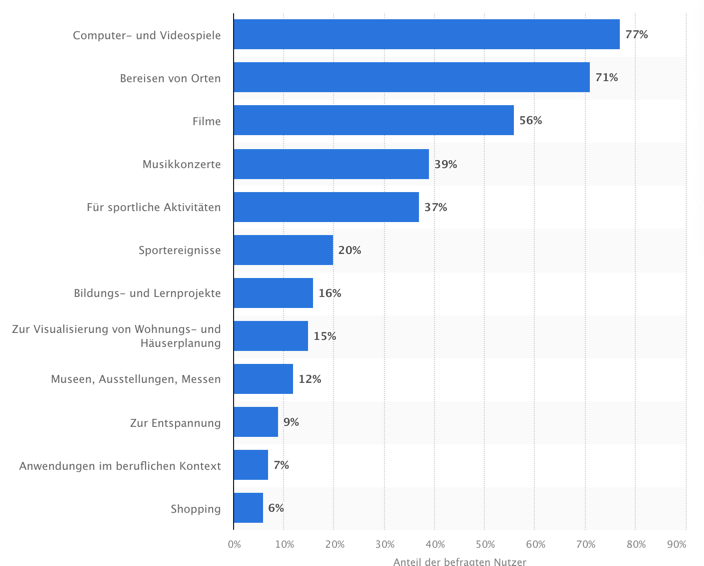
\includegraphics[scale=0.5]{pics/statistic_usage_vr}
    \caption{Anwendungsgebiete VR}
    \label{fig:statistic_usage_vr}
\end{figure}

Bei diesen VR Applikationen ist meist der Kopf getrackt und vielleicht auch Hände, Füße und Hüften.
Interconversions sind meistens aber die weitere interaktion mit der Umgebung.
Setzt einer sich auf einen Sessel wird er durchfliegen, außer er steht auch in der realen Wirklichkeit dort.

\section{Zielsetzung}\label{sec: objective}

Das Ziel von Beam VR ist die physische Realität und die virtuelle Realität zu kombinieren.
Im Falle Beam VR benützen wir hier einen Balken, welcher von einem Hochhaus wegsteht.
Dieser Balken soll in der physischen Realität und in der virtuellen Realität existieren und die gleiche Position einehmen.
Dadurch soll die Immersion entstehen, dass man wirklich auf einem Balken steht, welcher von einem Hochhaus wegsteht.
Auch, wenn man nur in seinem Wohnzimmer oder auch woanders ohne Gefahren auf einem Balken steht.
Beam VR ist nicht der Erfinder dieses Konzeptes.
Mehr dazu gibt es in der kommenden Umfeldanalyse.



\begin{spacing}{1}
\chapter{Umfeldanalyse}
\end{spacing}
% To Do
% Allgemeinerer Start           |
% Quellen nach jedem Absatz     |
% Rechtschreibung :(            |
%

Heutzutage kommen sich die virtuelle und die realle Realität immer näher.
Angefangen von Virtual Reality, wo sich der Benutzer mithilfe einer VR-Brille in eine fiktive Welt begeben kann.
Bis hin zu Augmented Reality, in welcher virtuelle Gegenstände und Strukturen in der reallen Welt angezeigt werden können.
Es gibt neben BeamVR auch noch viele andere verschiedene M\"oglichkeiten um diese Konzepte umsetzen zu können.


%Das Konzept der Synchronisation von einem Gegenstand über den zwei besprochenen Realitäten ist nicht neu.
%Einer der bekanntesten Implementierungen des Konzepts ist Richie's Plank Experience.

\section{Richie's Plank Experience}
\label{sec:richiesplankexperience}
Ein Projekt welches zu einem Teil das gleiche Thema wie BeamVR behandelt, heißt Richie's Plank Experience, welches von TOAST VR PTY. LTD. entwickelt wurde.
Es handelt sich um ein Virtual Reality Spiel, dass auf der PlayStation 4, Oculus Quest und f\"ur Microsoft Windows verf\"ugbar ist.
Bei der Playstation wird auf das Sony exclusive PlayStation VR zur\"uckgegriffen, während auf Windows entweder eine HTC Vive VR Brille oder die Valve Index verwendet werden kann.
~\cite{ToastGames_2021}

\subsection{Spielmodi}
\label{sec:richiesplankexperience_modes}
Richie's Plank Experience bietet dabei mehrere verschiedene Features in Form von Spielmodi an.
Diese Modi werden dem Spieler (\"ahnlich wie bei einer Stockwerkauswahl) in einem Aufzug dargestellt.
Wenn der Spieler einen Modus ausgewählt hat, fährt der Aufzug auf das Hochhausdach.
Dort befindet sich dann der entsprechende Aufbau für den Modus.
Zur Verfügung stehen hierbei die Modi Plank, Sky Brush, Ground, Hero Academy und der Easter Egg Modus Nightmare.
~\cite{ToastGames_2021_Steam}

Im ersten Modus, welcher Plank genannt wird, befindet sich der Spieler weit oben auf einem Hochhaus.
Nach der Auswahl wird angeboten, dass sich am Ende des Balkens eine Belohnung befindet.
Man kann zwischen einem leeren Balken, Kuchen, Donuts und Kuchen mit darin versteckten Spinnen auswählen.
Nun befindet sich vor dem Aufzug nur mehr der Balken mit der vorher getroffenen Belohnung und rundherum der Abgrund.
Die Donuts und die beiden Kuchen können entweder gegessen oder heruntergeworfen werden.
~\cite{ToastGames_2021_Steam}

In Sky Brush kann der Spieler, mithilfe eines kleinen Jetpacks, frei durch die Stadt fliegen.
Dabei wird eine Rauch-Spur hinterlassen welche, wie der Name des Modus schon andeutet, wie ein Pinsel in den Himmel malt.
Nun kann der Spieler, nach eigenem Belieben, verschiedene Kunstwerke erschaffen und betrachten.
~\cite{ToastGames_2021_Steam}

Bei Hero Academy kann der Spieler wieder zwischen mehreren Optionen auswählen.
Bei Fire Deck spielt man einen Superhelden welcher durch die Stadt fliegt und Feuer auf Häusern löschen muss.
Bei Air-Race fliegt man mit den Jetpacks durch Ringe welche als Checkpoints für ein Rennen dienen.
Wurden alle Ringe in richtiger Reihenfolge durchflogen, hat man das Rennen geschafft.
~\cite{ToastGames_2021_Steam}

Im geheimen Modus Nightmare, welcher mithilfe des Codes 666 erreicht werden kann, erlebt der Spieler eine kleine Abfolge von gruseligen Ereignissen.
~\cite{ToastGames_2021_VivePort}

\subsection{Setup}
\label{sec:richiesplankexperience_setup}

Damit man diese Modi, vor allem den Plank Modus, mit einem realen Balken spielen kann, muss mithilfe des Setups der Balken kalibriert werden.
Hierfür wird der Balken etwa in der Mitte der VR-Spielfläche platziert.
Nun sollten beide VR-Controller auf jeweils einem Ende des Balkens platziert werden, wie man auf der Grafik sehen kann.
\ref{fig:beam_length_measurement} %Balken Länge Einstellen

\begin {figure}
    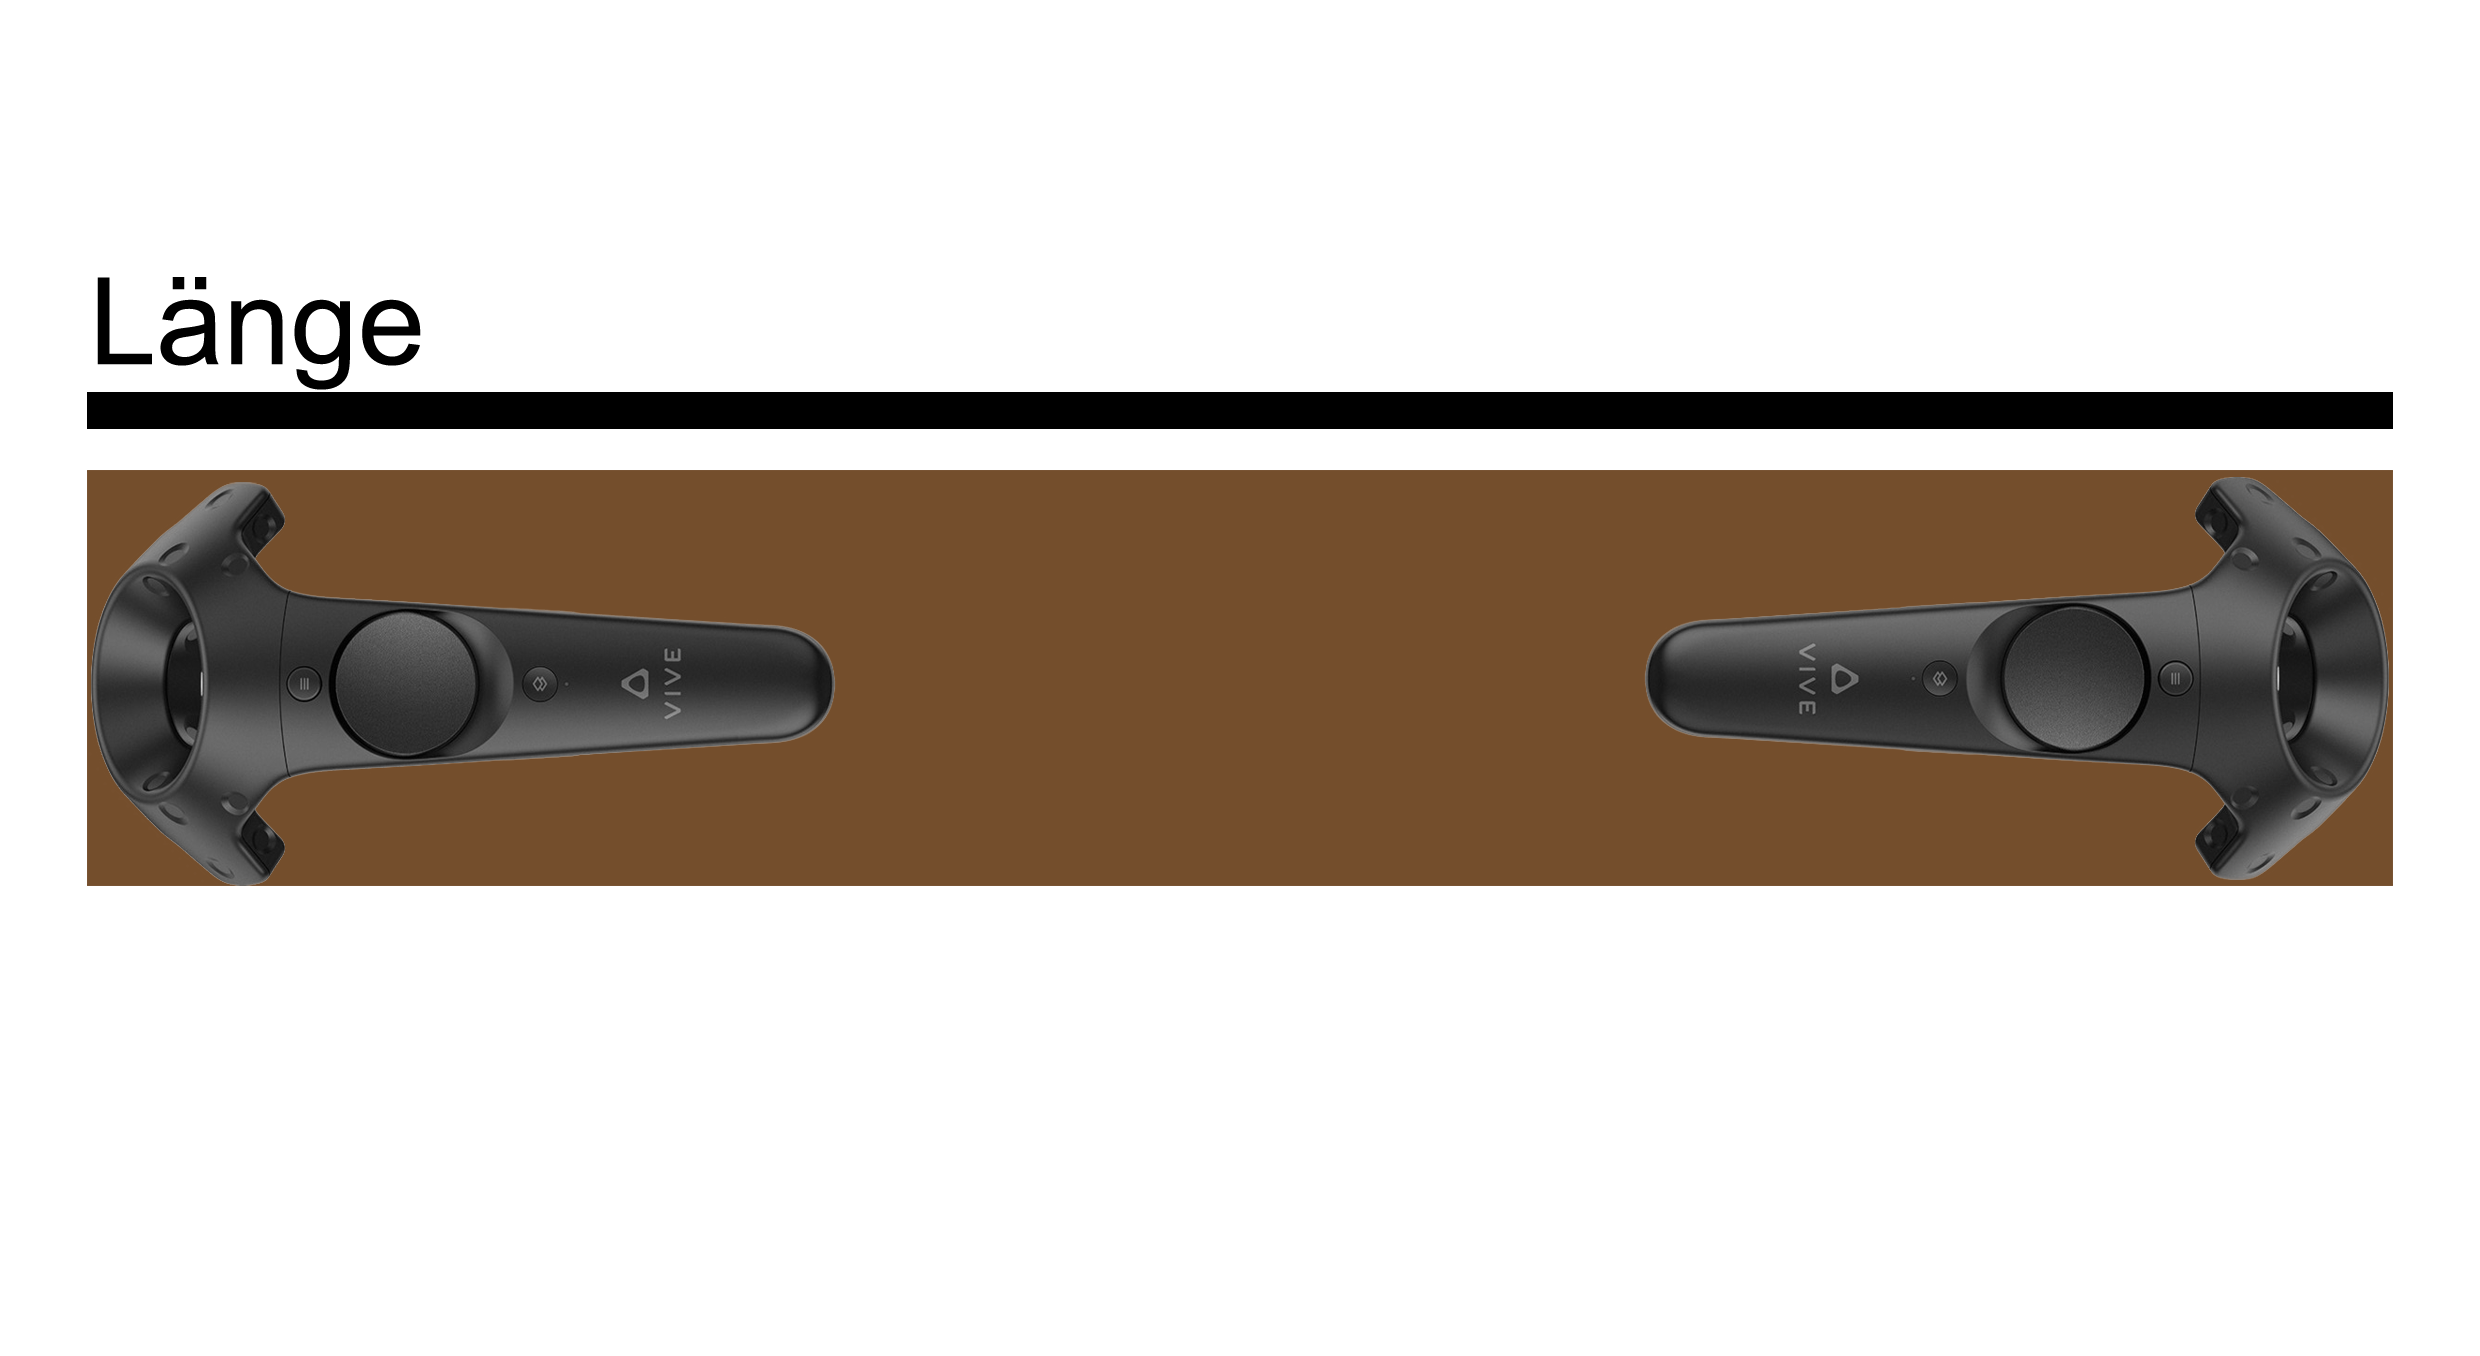
\includegraphics[scale=0.18]{pics/beam_length_measurement}
    \caption{L\"ange des Balken messen}
    \label{fig:beam_length_measurement}
\end {figure}

Dadurch weiß die Applikation wie lange der Balken ist.
Man wird aufgefordert den Trigger des Controllers zu drücken, welcher sich am Anfang des Balkens befindet, damit der Anfang und das Ende des Balkens bekannt gemacht wird.
%Grafik mit Setup Schritt 1



In Schritt zwei werden die Controller links und rechts vom Balken platziert und zeigen aufeinander.
Mit dieser Methode wird die Breite des Balkens gemessen.
%Grafik mit Setup Schritt 2
\ref{fig:beam_width_measurement} %Balken Länge Einstellen

\begin {figure}
    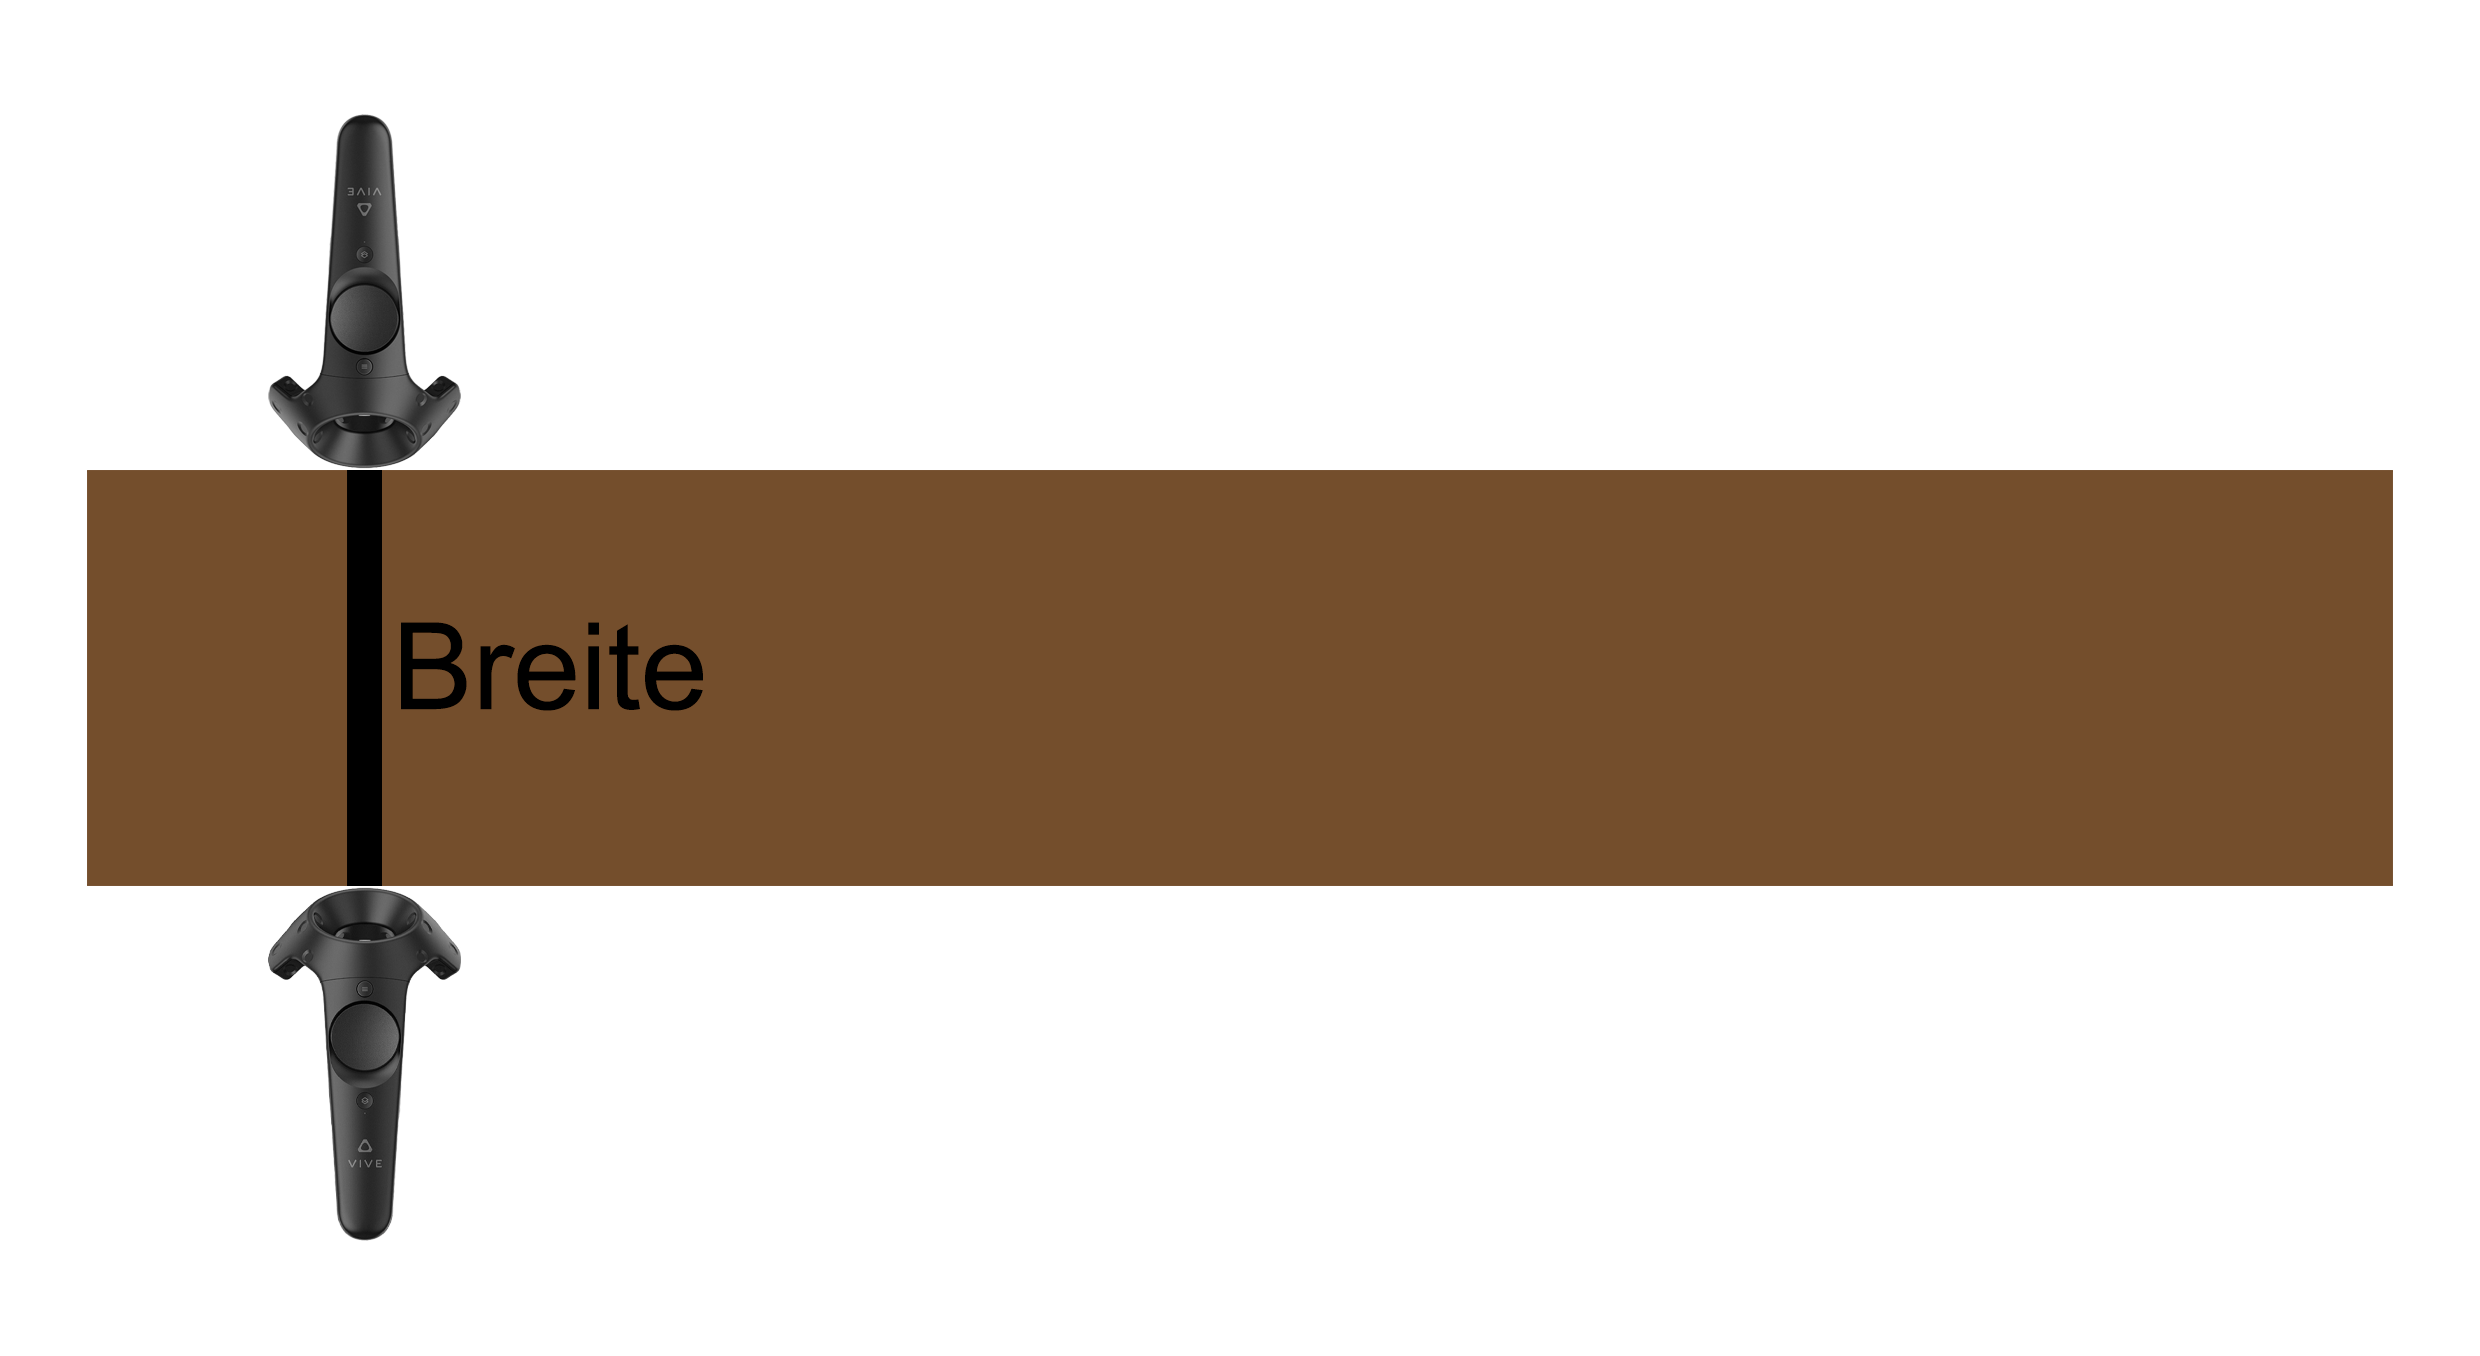
\includegraphics[scale=0.18]{pics/beam_width_measurement}
    \caption{Breite des Balken messen}
    \label{fig:beam_width_measurement}
\end {figure}


Nun ist das Setup abgeschlossen und der Balken wird richtig in der virtuellen Welt angezeigt.
~\cite{ToastGames_2021_Setup}

\subsection{Spielwelt}
\label{sec:richiesplankexperience_world}
Alle Spielmodi befinden sich in einer Stadt, welche aus einer Vielzahl an verschiedenen Gebäuden besteht.
Die Architektur ist sehr vielfältig und realistisch gehalten.
Zwischen den Bauwerken befinden sich Straßen welche mit verschiedenen Pflanzen, z.B. Bäumen, geschmückt sind.
Auf Fahrbahnen befinden sich Fahrzeuge, welche mit Schritttempo durch die Stadt fahren.

\ref{fig:richiesplankexperience_world} %Richies Plank Experience Spielwelt

\begin {figure}
    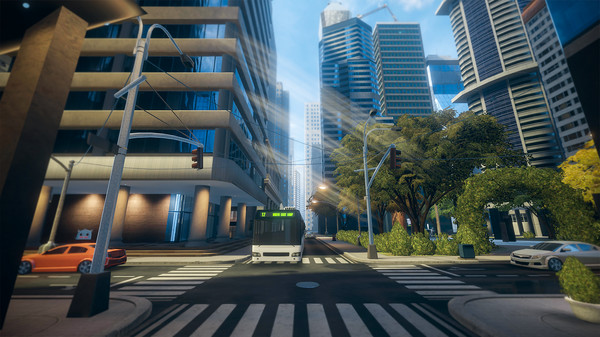
\includegraphics[scale=0.7]{pics/richiesplankexperience_world}
    \caption{Breite des Balken messen}
    \label{fig:richiesplankexperience_world}
\end {figure}


\section{VR Chat}
\label{sec:vrchat}
VR Chat befasst sich ebenfalls mit einer \"anlichen Thematik wie BeamVR.
In diesem Fall wird jedoch kein Balken sondern der ganze K\"orper des Benutzers mit Controllern getrackt.

\subsection{Spielprinzip}
\label{sec:vrchat_principle}
Wie der Name schon sagt, handelt es sich um eine in VR ausf\"uhrbare Anwendung.
Da aber nicht jeder eine VR Brille besitzt, kann man auch eine Desktop Variante spielen, welche mit Maus und Tastatur bedient wird.
In diesem Programm geht es haupts\"achlich um die Interaktion mit unbekannten Spielern aus dem Internet,
welche ebenfalls diese Applikation verwenden.
Wer jedoch mit freunden Spielen möchte, kann das nat\"urlich auch.
Eine Vielzahl an, von Spielern erstellten, Welten und Spielmodi erwarten einen und es kommen weiterhin Neue dazu.
Von einer Runde Capture the flag im Weltall, bishin zu einem entspannenden Abend an einem Lagerfeuer im Wald, ist alles möglich.
~\cite{VRChat_2021_Steam}

\subsection{Verwendungs M\"oglichkeiten}
\label{sec:vrchat_usecases}
Es gibt extrem viele m\"oglichle Verwendungszwecke für eine Applikation wie VR Chat.
Die 4 Gr\"oßten sind jedoch, die Option neue Freunde im Internet kennenzulernen, eigene Welten zu erschaffen, sein digitales Aussehen selber bestimmen zu k\"onnen und Teil einer riesigen Community zu werden.
~\cite{VRChat_2021})

VR Chat ist eine soziale Platform auf welcher sich tausende Spieler gleichzeitig befinden, diese Interagieren in Form von Gespr\"achen oder Gesten miteinander.

Die Entwickler stellen einem die n\"otigen Funktionen zur Verf\"ugung um eigene Welten zu kreiren. Die Spieler fertigen neue Spielmodi wie z.B. Capture the flag, Lasertag, Theaterauff\"uhrungen, etc. an und errichten passende Umbegungen dazu.

Wem die standard Spielermodelle nicht gefallen, kann einfach mithilfe des Steam Workshops und Tools wie Ready Player Me, Tafi oder MakeAvatar, weitere Modelle downloaden und sofort im Spiel benutzen.
Durch dieses Feature f\"uhlt sich die Applikation sofort viel pers\"önlicher an, da man sich mit den Modellen gut identifizieren kann.
~\cite{VRChat_2021_AvatarCreator}

\subsection{Full Body Tracking}
\label{sec:vrchat_fullbodytracking}
Wer die n\"otigen Tracker besitzt, hierbei handelt es sich gleich wie bei BeamVR um z.B. die Vive Tracker, kann sogar seinen K\"orper und seine Beine in dem Spiel tracken.
Dafür sind nicht mehr als 3 Schritte notwendig.
~\cite{VRChat_2021_FullBodyTracking}

Als erstes muss man in das Men\"u des Spieles gehen und auf den Kalibrieren Knopf dr\"ucken.

Als n\"achstes wird ein Spielermodell ausgew\"ahlt.
Dieses wird darauf hin in einer T-Pose vor dem Spieler ersichtlich sein.
Weiters werden mithilfe von weißen Punkten die Positionen der Tracker in der Applikation angezeit, diese Sollten nun vern\"unftig platziert werden..

Als Letztes muss man nur noch die Eingabe best\"atigt werden und das Spielermodell macht die Bewegungen des Spielers nach.

%\subsection{Avatar Erstellung}s
%\label{sec:vrchat_avatarcreation}


\begin{spacing}{1}
\chapter{Technologien}\label{chapter:tech}
\end{spacing}
\section{Hardware}
\lipsum[5-12]

\subsection{VR Headset}
\lipsum[5-12]

\subsection{VR Controller}
\lipsum[5-12]

\subsection{Tracker}
\lipsum[5-12]

\subsection{Lichtboxen}\label{sec:lighthouse}
\lipsum[5-12]

\subsection{Wireless Adapter }
\lipsum[5-12]

\section{Software}

\subsection{Game Engine}

Es gibt mehrere Games Engines mit welchen eine VR Applikation geschrieben werden kann.
In Abbildung~\ref{fig:game_engine_marketshare} kann man den market share verschiedener Engines sehen.
Diese Daten sind aber mit vorsicht zu genießen, da das Skript welche diese Daten geliefert hat nach einigen Kriterien handelt.
Siehe~\cite{REDDIT_2018}.

\begin{figure}
    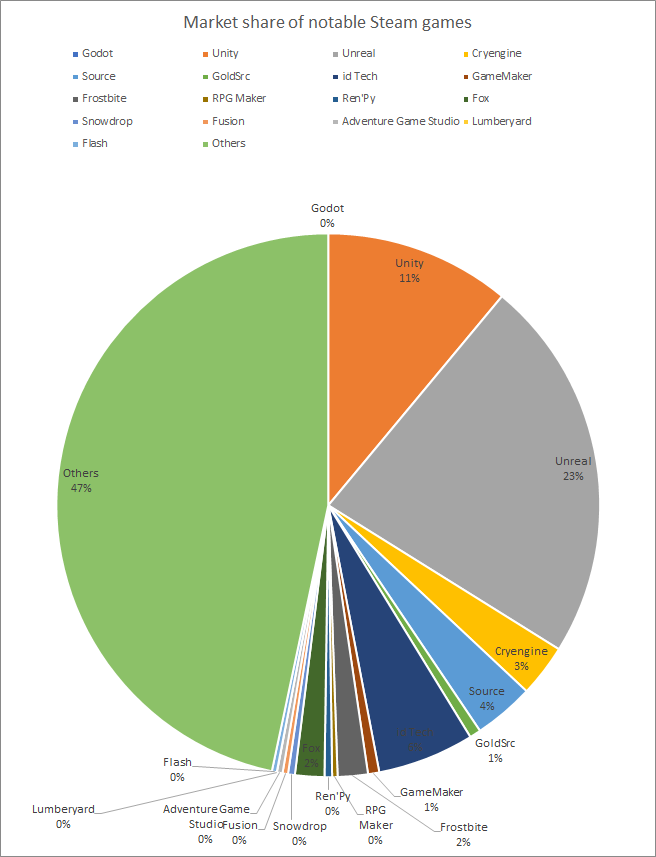
\includegraphics[scale=0.5]{pics/game_engine_marketshare}
    \caption{Game Engine Market-share}
    \label{fig:game_engine_marketshare}
\end{figure}

\subsubsection{Unity}

Unity ist eine Game Engine welche erstmals eine Apple exklusive Game Engine war und von Unity Technologies entwickelt worden ist.
Die Engine wurde weiter entwickelt und kann heute auch auf Windows und auf der Linux plattform benützt werden.
Die Engine ist gratis und wird von vielen als Einsteiger Engine beschrieben.
Auch sie eine Einsteiger Engine genannt wird heißt das nicht, dass sie in keinen professionellen Bereich benützt wird.
Viele bekannte Spiele wurden mit der Unity Engine entwickelt.
Im Besonderen sind viele Handyspiele mit dieser Engine entwickelt.
Spiele wie Pokemon GO, Among us und Hearthstone wurden in der Unity Engine entwickelt.

Vorteile:

\begin{itemize}
    \item Gratis Lizenz für persönlichen Nutzen und für Unternehmen mit unter 100000\$ Einkommen
    \item Programmierbar in der C# Programmiersprache
    \item Es kann fuer alle moeglichen Plattformen ein Programm geschrieben werden
    \begin{itemize}
        \item IOS
        \item Android
        \item Windows
        \item Linux
        \item usw.
    \end{itemize}
    \item verfügbaren Asset-store mit vielen verschiedenen fertigen Assets
\end{itemize}

Nachteile:

\begin{itemize}
    \item weniger Market-share~\ref{fig:game_engine_marketshare}
    \item geschlossener Source Code
\end{itemize}

\subsection{VR Plugin}
\lipsum[5-12]

\subsection{Steam}
\lipsum[5-12]

\subsection{Vive Wireless}
\lipsum[5-12]

\subsection{Final IK Plugin}
\lipsum[5-12]

\subsection{IDE}
\lipsum[5-12]

\subsection{Modellierung}
\lipsum[5-12]


\begin{spacing}{1}
\chapter{Umsetzung}\label{chapter:implementation}
\end{spacing}
\section{3d Welt}\label{sec:3d-world}
\setauthor{Florian Beckerle}
Jedes Spiel besitzt eine Spielwelt.
Dabei ist es egal ob es sich um eine 3D oder 2D Applikation handelt.
Unter den Begriff Spielwelt fällt die Umgebung in welcher, sich der Spieler befindet.
Es gibt hierbei so gut wie keine Einschränkungen in Bezug auf Kreativität, egal ob die digitale Welt nun ein riesiger Ring, der im Weltall schwebt,
oder eine verlassene Großstadt in einer postapokalyptischen Welt ist, siehe Abb. ~\ref{fig:3d_environment_destiny2}.
~\cite{GamesRadar_HaloRing_2022}



%% this image and the next are not working. see issue #1

\begin{figure}
    \centering
    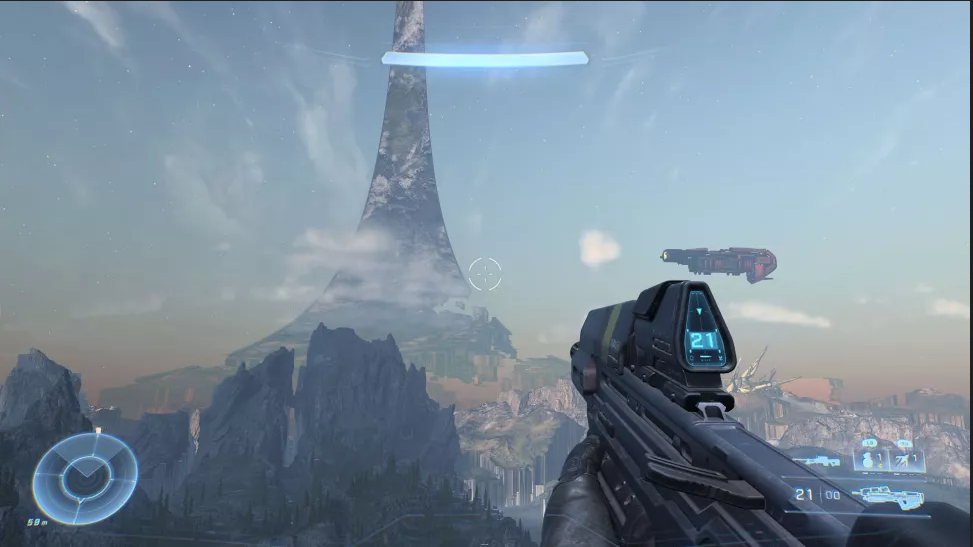
\includegraphics[scale=0.4]{pics/3d_welt_halo_ring}
    \caption{3D Welt - Halo}
    \label{fig:3d_environment_halo}
\end{figure}


%% Grafik für Destiny 2 Locations noch einbinden (Seite für Quelle lädt grade nicht Bungie.net)

\begin{figure}
    \centering
    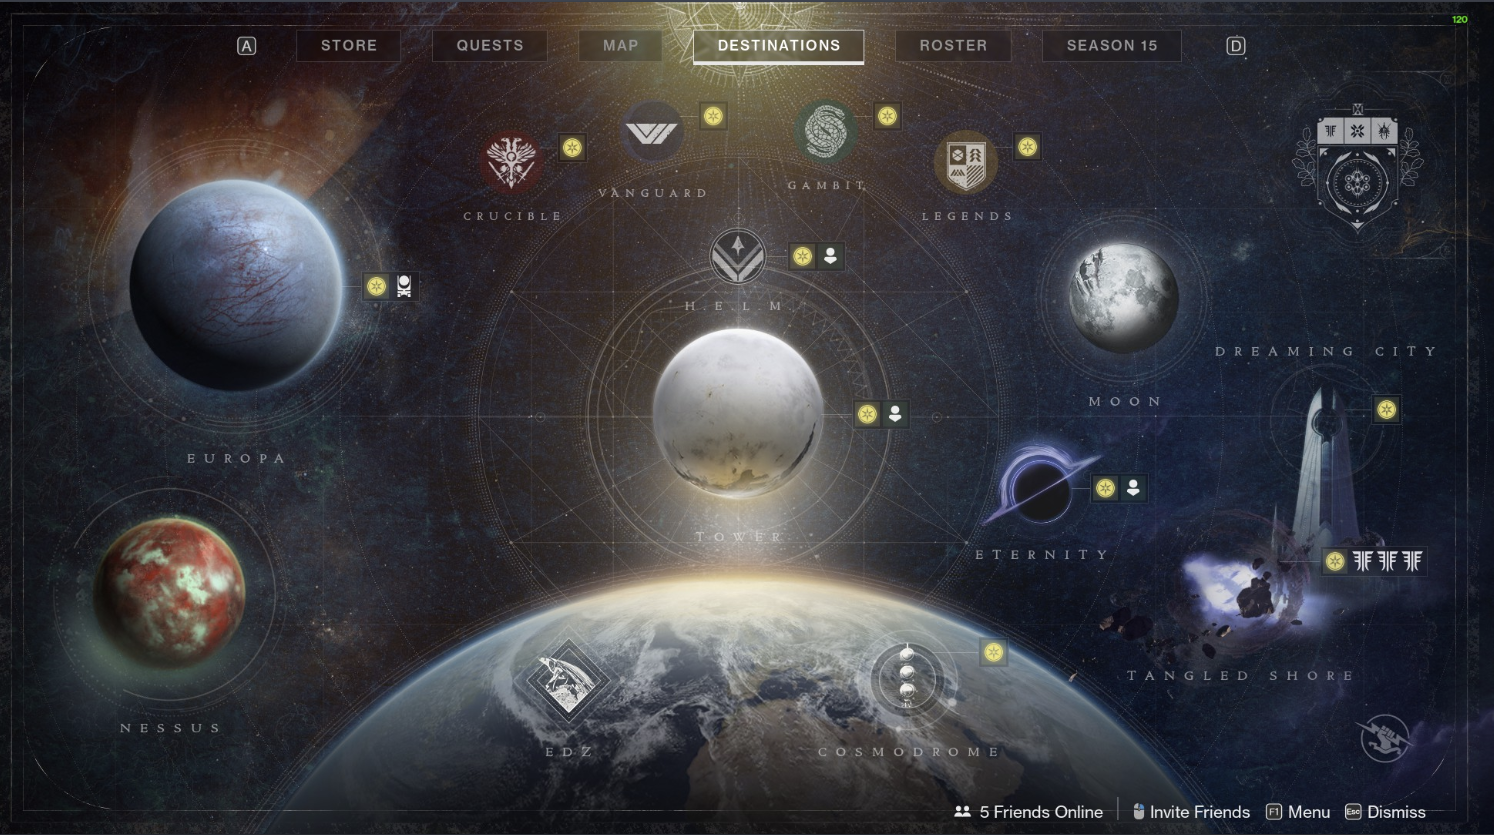
\includegraphics[scale=0.3]{pics/3d_welt_destiny_planets}
    \caption{3D Welt - Destiny 2}
    \label{fig:3d_environment_destiny2}
\end{figure}

Spielehersteller bauen die Spielwelten so auf, wie es am besten zu der Vision des Spieles passt.
Gleichzeitig wird darauf geachtet, dass sich die Umgebung nicht langweilig oder leer anfühlt.
Hierfür wird Environmental Storytelling verwendet.
Darunter versteht man das Platzieren von Gegenständen und Objekten,
welche dem Spieler eine kleine Geschichte erzählen.
Das passiert jedoch nicht über Sprache sondern einfach nur über die Platzierung und das Aussehen.
Ein Beispiel hierfür w\"are das Bild von Cayde-6 (ein Charakter aus Destiny 2), welches in einem Restaurant platziert wurde.
Cayde ist einer der drei Anführer der Vanguard, welche eine Ansammlung an Guardians (Spielern und NPC) ist und gegen das Böse kämpft.
In Forsaken starb Cayde jedoch und viele trauerten um ihn, als Gedenken wurde dieses Bild aufgehängt.
~\cite{GameDeveloper_2022}

\begin {figure}
    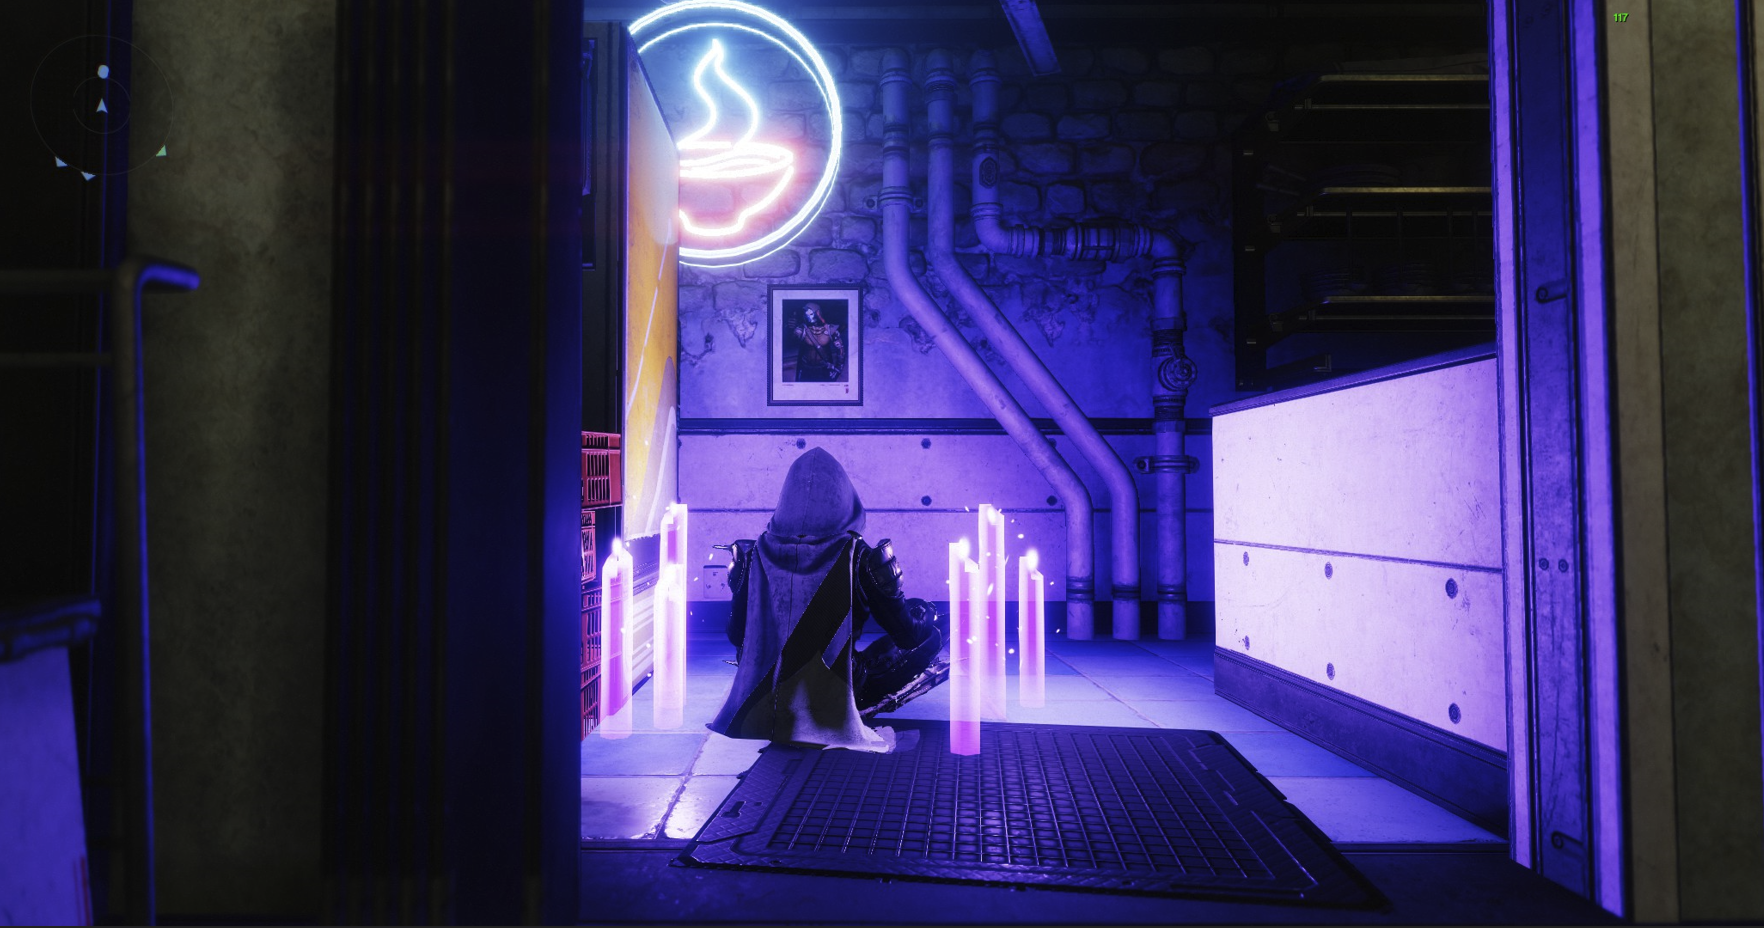
\includegraphics[scale=0.3]{pics/3d_welt_destiny2-environmental-storytelling}
    \caption{Environmental Storytelling '-' Destiny 2 Cayde}
    \label{fig:3d_environmental_storytelling_destiny2}
\end {figure}


\subsection{City Grid System}\label{subsec:city-grid-system}
\setauthor{Florian Beckerle}
Um die Gestaltung der Welt in BeamVR zu erleichtern, wurde ein Grid System verwendet.
Dafür ist die Stadt in ein Raster aufgeteilt, an welchem sich alle Objekte der Welt auf allen 3 Achsen (x,y,z) orientieren.
Unity stellt, wie in Abb. ~\ref{fig:grid-system-unity} zu sehen, so ein Grid Snapping System zur Verf\"ugung.
Daher wurde f\"ur BeamVR am Anfang der Modellierungsphase eine bestimmte Grid-Size festgelegt,
an welche die Grundfl\"achen der Geb\"aude und die Straßen
angepasst wurden.

\begin {figure}
    \centering
    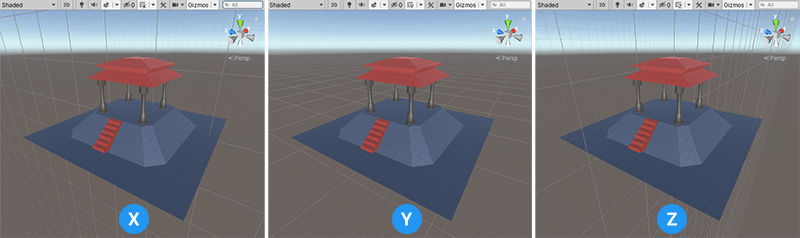
\includegraphics[scale=0.5]{pics/unity-grid-snapping}
    \caption{Unity '-' Grid Snapping System}
    \label{fig:grid-system-unity}
\end {figure}

Wenn man die Grid Size, also die Gr\"osse des Rasters \"andern m\"ochte, muss man zuerst im Editor das Grid and Snap Fenster öffnen.
Als n\"achstes findet man unter dem Bereich World Grid ein Attribut namens Size, wo man die X, Y und Z Achsen frei und unabh\"angig voneinander umskalieren kann, siehe Abb. ~\ref{fig:grid-size-unity}.
~\cite{Unity_GridSnapping_2022}

\begin {figure}
    \centering
    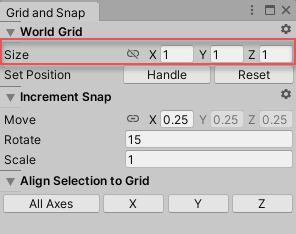
\includegraphics{pics/unity-grid-snapping-size}
    \caption{Unity - Grid Snapping Size}
    \label{fig:grid-size-unity}
\end {figure}



\subsection{Stadt}\label{subsec:city}
\setauthor{Florian Beckerle}
Jede Stadt hat viele verschiedene Strukturen wie zum Beispiel Sehensw\"urdigkeiten, Bauwerke und Einrichtungen wie Kinos, Theater oder Restaurants.
F\"ur BeamVR wurden daher insgesamt \"uber 34 Geb\"aude Modelle erstellt, um eine Vielfalt in der Umgebung zu erreichen, siehe Abb. ~\ref{fig:beamvr_building-variety}.

\begin {figure}
    \centering
    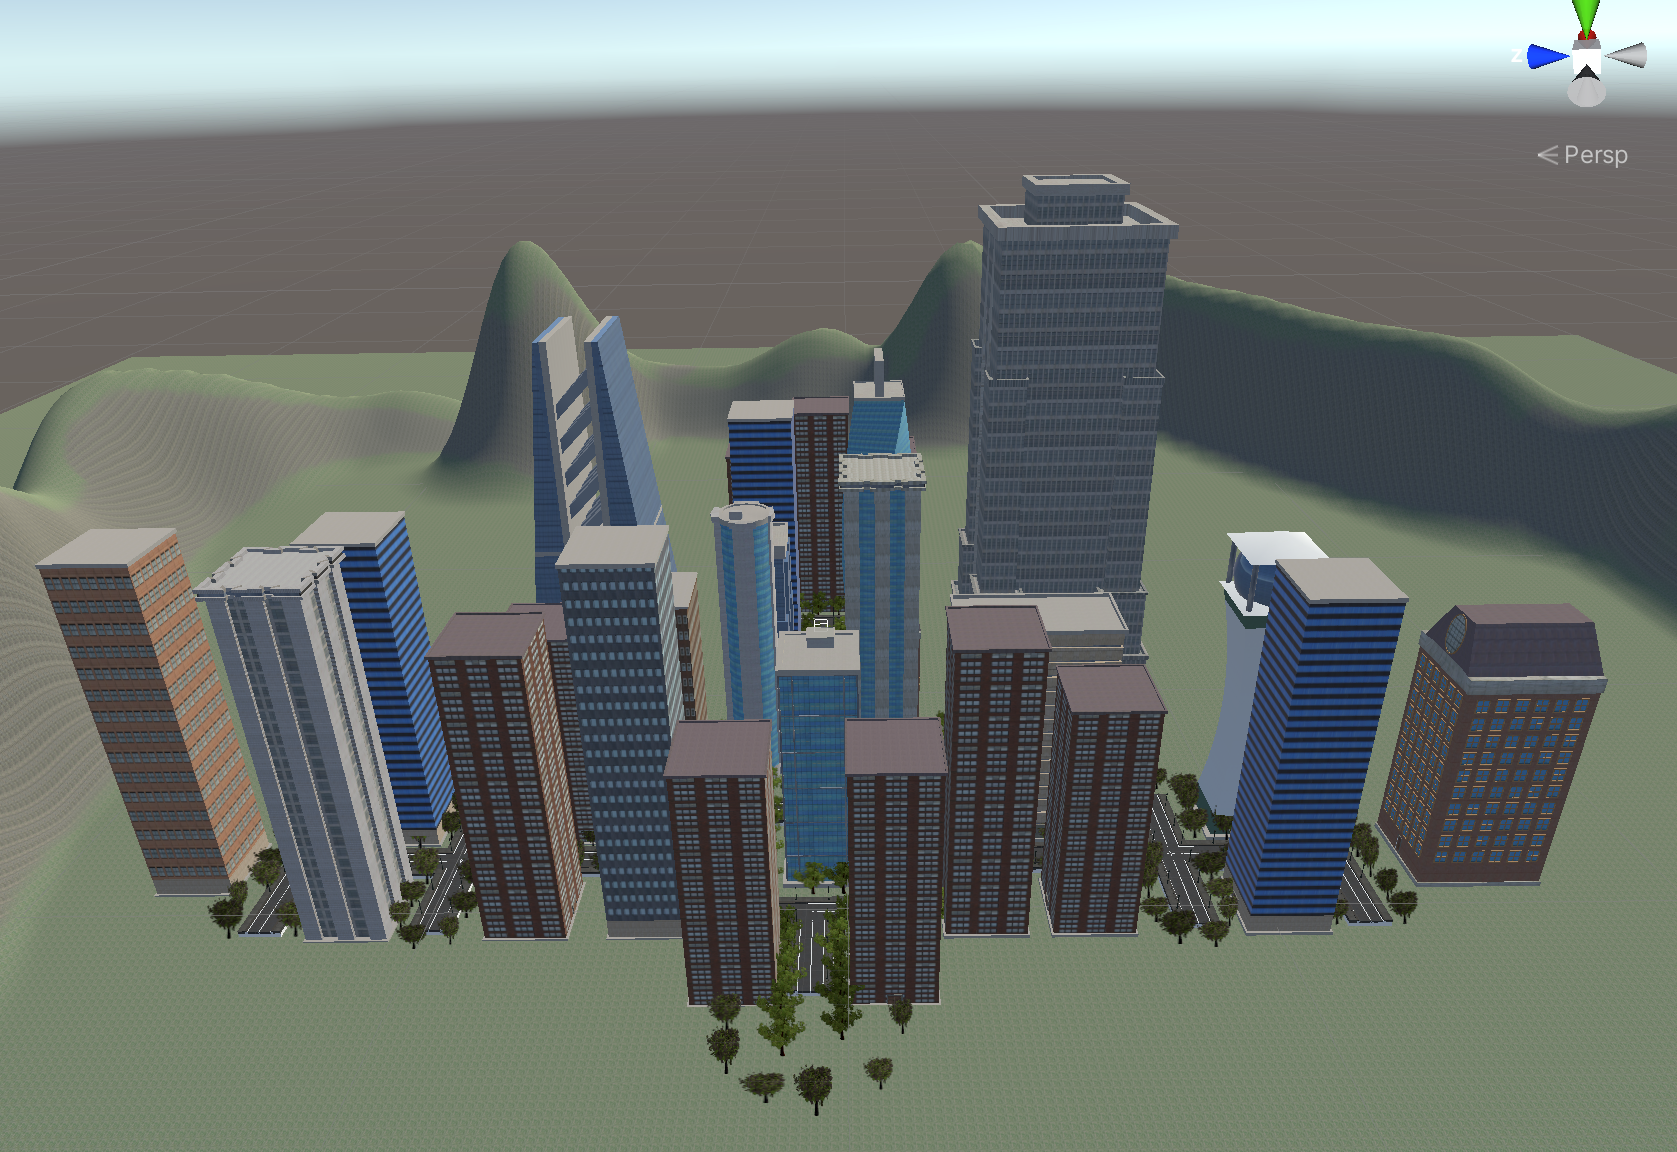
\includegraphics[scale=0.18]{pics/beamvr_building-variety}
    \caption{Beam VR - Building Overview}
    \label{fig:beamvr_building-variety}
\end {figure}

Die Stadt wurde so entworfen, dass nur die für den Spieler sichtbaren Objekte wirklich existieren, wie auf der Abb. ~\ref{fig:beamvr_building-variety} zu erkennen ist.
Bei richtiger Umsetzung scheint es für den Anwender dennoch so, als w\"are dieser in einer kompletten Spielwelt.
Um die Performance des Spieles zu verbessern, wurde dieser Trick in BeamVR angewandt, da unn\"otige Objekte nicht gerendert oder berechnet werden m\"ussen.
Bei gr\"oßeren Projekten spart das nicht nur Zeit sondern auch Ressourcen.
Bei BeamVR wurde diese Technik angewandt, um die Frames per Second zu erh\"ohen.

\subsection{Tag Stadt}\label{subsec:day-city}
\setauthor{Florian Beckerle}
Es wurden 17 der 34 unterschiedlichen Geb\"aude f\"ur diese Map modelliert, siehe Abb. ~\ref{fig:beamvr_building-variety}.
Der Fokus bei der Gestaltung der Bauwerke lag darauf, dass diese m\"oglichst realistisch aussehen und dennoch nicht zu rechenaufwendig in der Darstellung sind.
Daher wurden Texturen verwendet, um kleinere Details an den Fassaden darzustellen, statt diese zu modellieren.
Das gleiche Prinzip wurde bei der Apocalypse Map verwendet, siehe Abschnitt ~\ref{subsec:apocalypse-city}.
Die Texturen stellen Fassaden aus Stein und Glas dar.
Ein weiterer wichtiger Punkt bei der Planung der Stadt war es auch, dass der Spieler nicht aus der Stadt hinaus schauen kann und die Illusion aufrecht erhalten bleibt.
Daher wurden alle umliegenden Bauwerke mindestens 3 Meter h\"oher gemacht als das Geb\"aude, auf dem sich der Spieler befindet, siehe Abb. ~\ref{fig:beamvr_building-heights}.

\begin {figure}
    \centering
    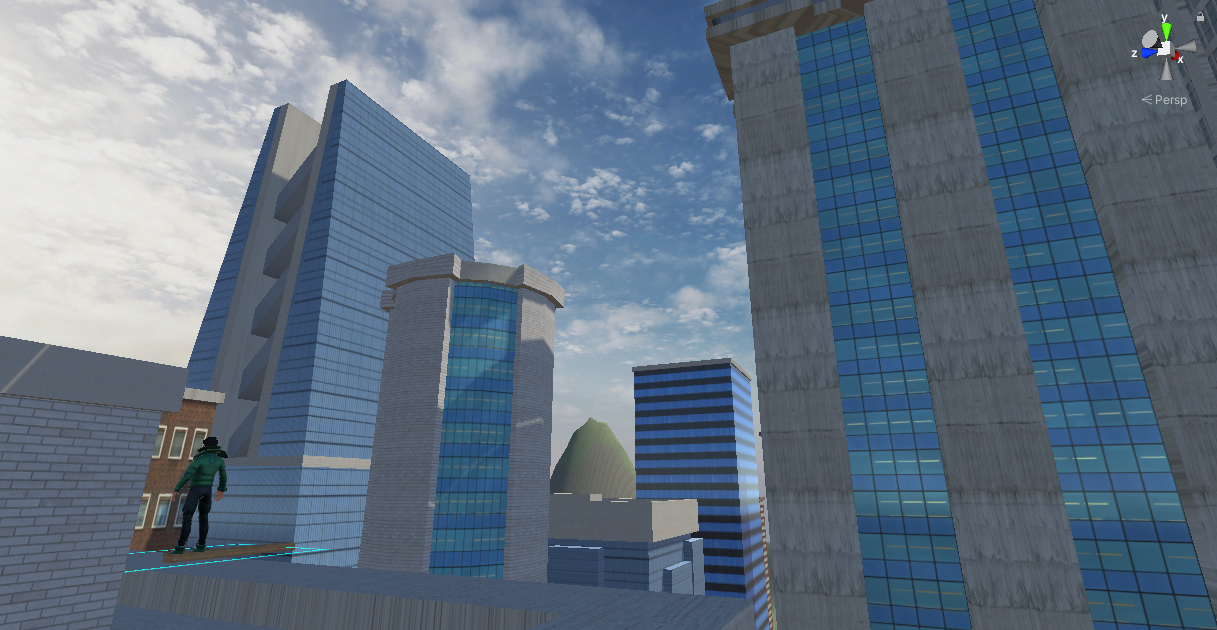
\includegraphics[scale=0.5]{pics/beamvr_city_day_heights}
    \caption{Beam VR - Building Heights}
    \label{fig:beamvr_building-heights}
\end {figure}

\subsection{Nacht Stadt}\label{subsec:night-city}
\setauthor{Florian Beckerle}
In der Nacht Version der Stadt wurde die Skybox angepasst.
Diese zeigt nun einen Sternenhimmel.
Es handelt sich hierbei um eine Sphere oder Box, welche sich um die Spielwelt befindet.
Sie wird dazu benutzt, um einen Himmel oder andere Umgebungen,
in Form von Texturen darstellen zu können, ohne dass diese als Modelle existieren.
Zus\"atzlich wurde die Belichtung der Scene auf ein bl\"auliches Licht eingestellt und die Laternen in den Straßen
haben noch eigene Lichtquellen, siehe Abb. ~\ref{fig:beamvr_night_map_lighting}.

\begin {figure}
    \centering
    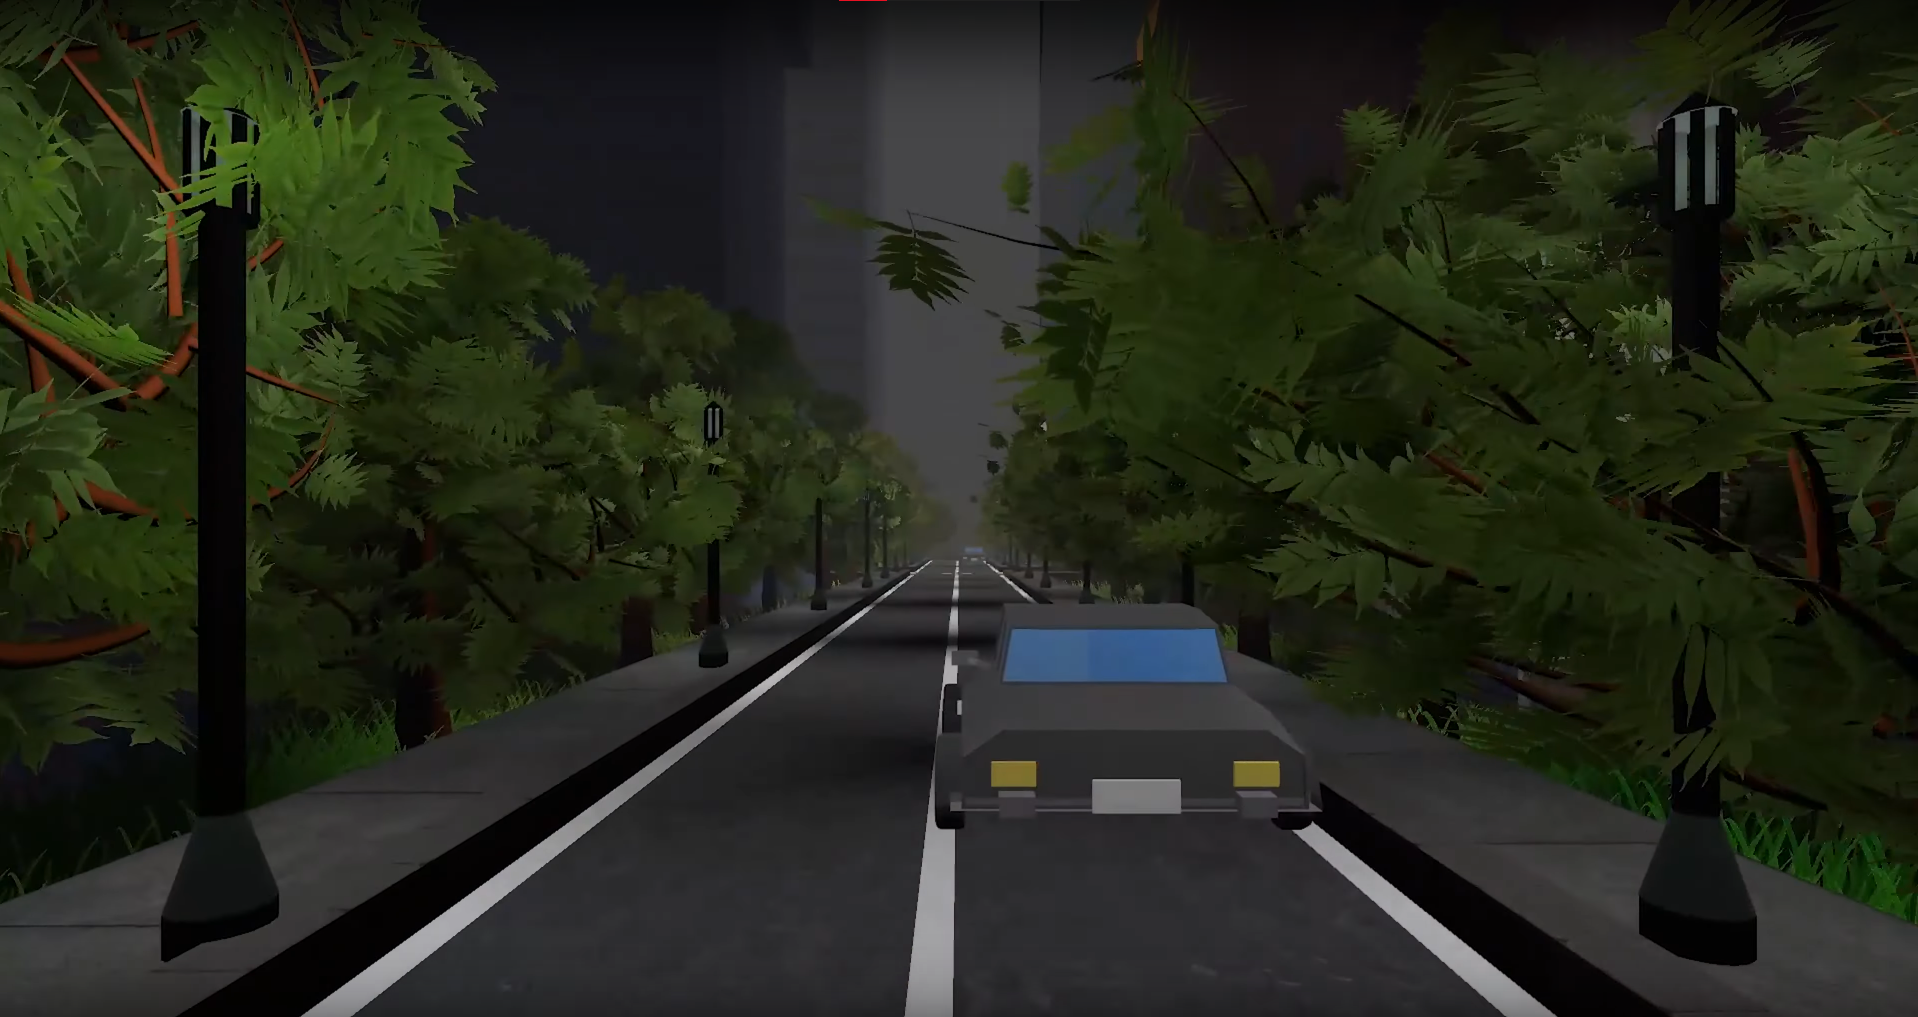
\includegraphics[scale=0.3]{pics/beamvr_night_overview}
    \caption{Beam VR - Night Map Lighting}
    \label{fig:beamvr_night_map_lighting}
\end {figure}

\subsection{Apocalypse Stadt}\label{subsec:apocalypse-city}
\setauthor{Florian Beckerle}
F\"ur diese Umgebung wurden alle Geb\"aude nocheinmal \"uberarbeitet.
Statt der intakten Glasfassaden werden nun barrikadierte Fenster und Ziegelsteine ohne Verputz f\"ur die Bauwerke verwendet, siehe Abb. ~\ref{fig:beamvr_damaged_texture}.
Durch diese \"Anderung sieht die Stadt verlassen und postapokalyptisch aus.
Um den Effekt noch zus\"atzlich zu verst\"arken, wurden die Bauwerke in eine Schieflage gebracht, sodass es aussieht, als w\"urden diese gleich zusammenbrechen.
Das Gel\"ande wurde mit neuen Sandstein Texturen und D\"unen in eine W\"uste umgewandelt.
Die Planzen und B\"aume wurden durch ausgetrocknete B\"usche ausgetauscht, damit die Welt ein trostloses Aussehen erhält, siehe Abb. ~\ref{fig:beamvr_apocalypse_map}.

\begin {figure}
    \centering
    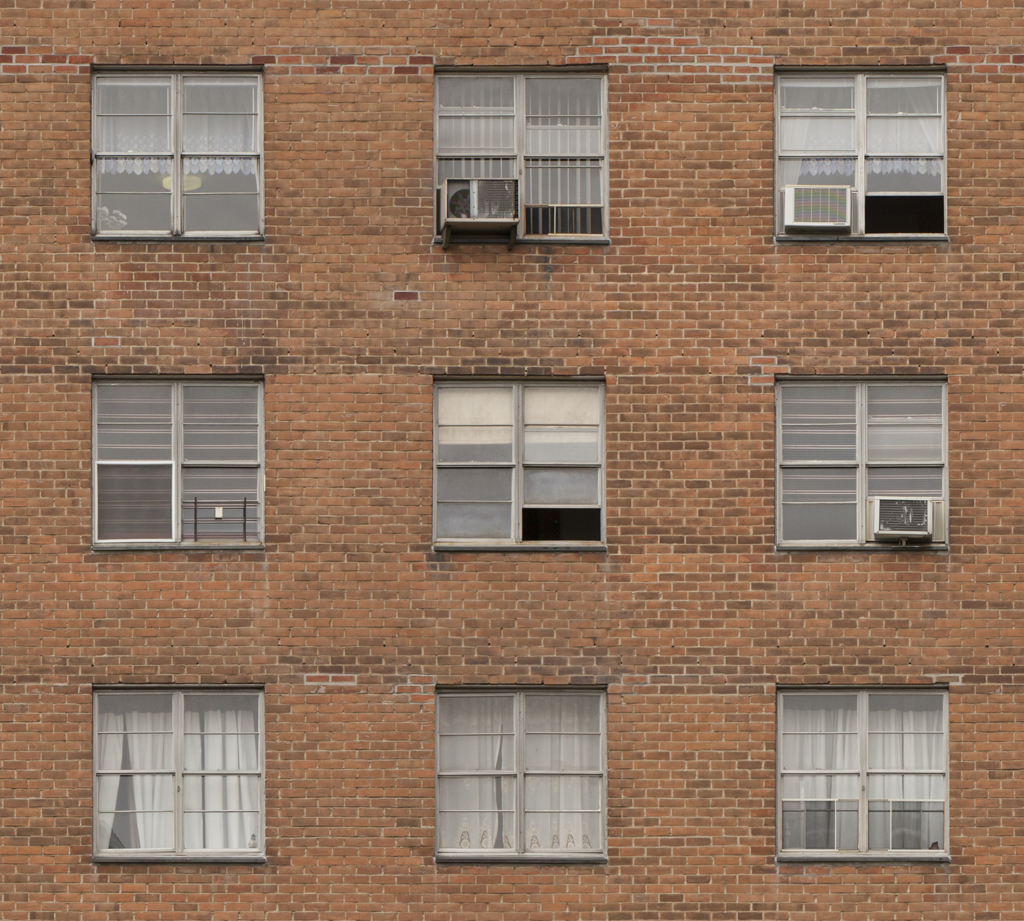
\includegraphics{pics/beamvr_damaged_texture}
    \caption{Beam VR - Damaged Texture}
    \label{fig:beamvr_damaged_texture}
\end {figure}

\begin {figure}
    \centering
    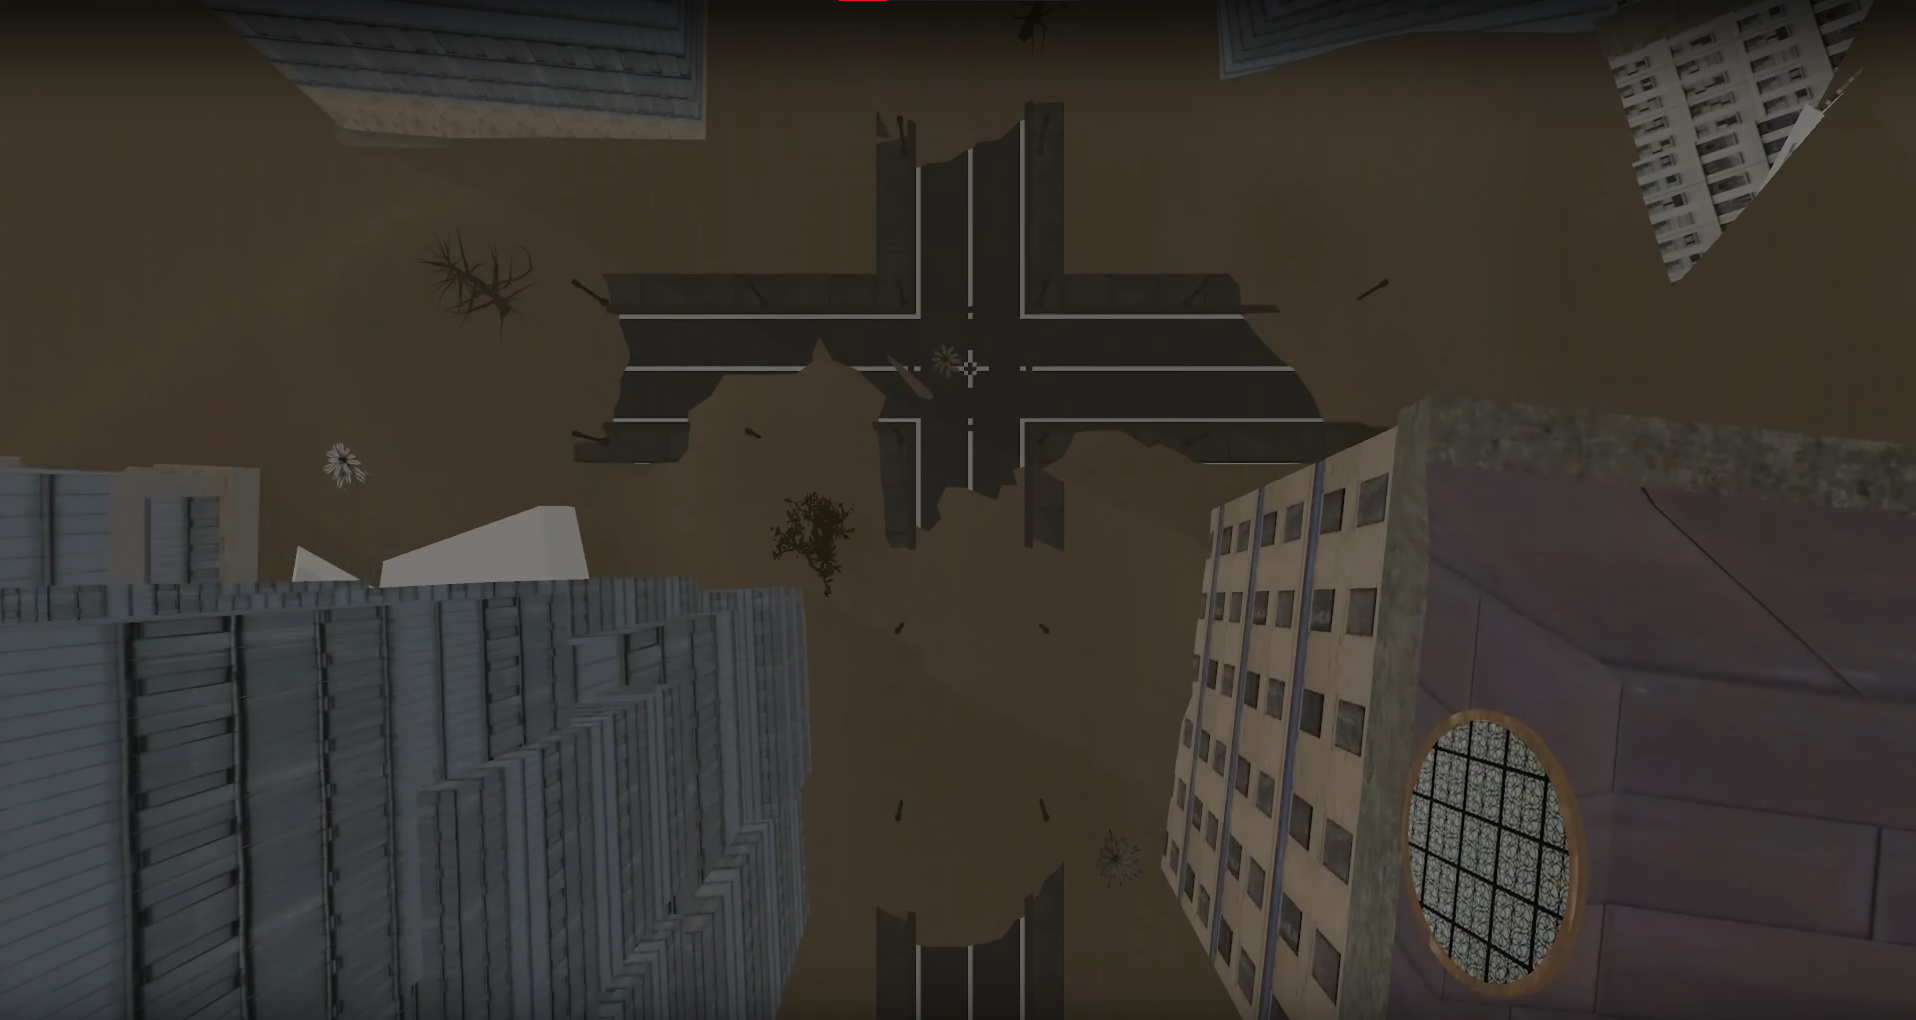
\includegraphics[scale=0.3]{pics/beamvr_apocalypse-overview}
    \caption{Beam VR - Apocalypse Map}
    \label{fig:beamvr_apocalypse_map}
\end {figure}

\section{Sound Design}\label{sec:sound}
\setauthor{Florian Beckerle}
Ohne Sound Design würden die Maps von BeamVR unrealisitsch wirken, da in einer Stadt Lärm an der Tagesordnung steht.
In der virtuellen Umgebung der verwendeten Game Engine existieren anfangs keine Geräusche, diese m\"ussen von den Entwicklern selber erstellt und eingef\"ugt werden.


Es gibt viele verschiedene Arten Sound Design zu benutzen wie zum Beispiel die Ger\"ausche, die der Anwender selbst in der virtuellen Welt verursacht.
Wenn sich der Spieler bewegt, sollten Fußstapfen zu h\"oren sein.
Diese klingen je nach Bodentyp unterschiedlich.
Besteht der Boden aus Holz, wird man ein h\"olzernes Klopfen und Knarren h\"oren.
Ist der Boden jedoch mit Gras bedeckt, wird ein Rascheln abgespielt.
Zus\"atzlich wird der gesteuerte Charakter außer Atem sein, wenn gelaufen wurde oder gerade ein Sprung ausgef\"uhrt wird.
Das wird mithilfe von Atem-Geräuschen umgesetzt.

Bei Umgebungen ist es wichtig, dass die Welt nicht leer klingt, sondern mit situationsbedingten Hintergrundger\"auschen voller Leben erscheint.
Es gibt jedoch auch Situationen, in denen gezielt wenig Umgebungsger\"ausche benutzt werden, um zum Beispiel eine W\"uste oder eine verlassene Stadt noch einsamer und trostloser darzustellen.

Um die Stimmung noch genauer steuern zu k\"onnen, kann Musik benutzt werden.
Wenn der Spieler auf einem Pferd durch eine Weide reitet, kann eine dramatische und inspirierende Musik benutzt werden, um den Moment noch besser und cinematischer wirken zu lassen.

Die Informationen für die Absätze wurden hier gefunden ~\cite{GK_Media_Factory_Sound_Design_2022}.

\subsection{Apocalypse}\label{subsec:apocalypse-background-sound}
\setauthor{Florian Beckerle}
Die Musik in der Apocalypse Map ist stark an das Horror Genre angelegt.
Die Melodie ist jedoch nicht wirklich existent, stattdessen existiert ein durchgehendes pfeifendes Ger\"ausch, welches unterbewusst das Spannungslevel erh\"oht.
Der Spieler f\"uhlt sich etwas unbehaglich und alleine.
Dadurch wirkt die Stadt, neben den br\"ockelnden H\"ausern, zus\"atzlich noch mehr verlassen.

Da die Sicht in dieser Map stark durch einen gelblichen Nebel, der wie ein Sandsturm wirkt, eingeschr\"ankt ist, kann man im Hintergrund den Wind pfeifen h\"oren.

\subsection{City}\label{subsec:day-night-background-sound}
\setauthor{Florian Beckerle}
Die Hintergrundger\"ausche der Tag und Nacht Version der Stadt sind sehr \"ahnlich.
Der Spieler kann Motorr\"ader und Autos auf den Straßen vorbeifahren h\"oren.
Hin und wieder kann man Menschen, die man nicht sehen kann, bei kurzen Gespr\"achen miteinander zuh\"oren und ein Kind husted im Hintergrund.

\subsection{Event}\label{subsec:building-collapse-sound}
\setauthor{Florian Beckerle}
Um spezifische Events, also bestimmte Dinge, welche in der Welt passieren, f\"ur den Benutzer besser erkennbar zu machen, wurden zus\"atzlich Ge\"ausche eingef\"ugt.
Auf der Apocalypse Map sind zusammenbrechende Geb\"aude zu h\"oren, um die schlechte Instandhaltung der verlassenen Stadt erneut zu verdeutlichen.
Aber wenn der Benutzer genauer hinsieht kann man, wenn diese Sounds h\"orbar sind, auch tats\"achlich eine kleine Auswahl an Bauwerken br\"ockeln sehen.

\section{Effects}\label{sec:effects}
\setauthor{Florian Beckerle}
Unity bietet verschiedene M\"oglichkeiten, um das Aussehen der Applikation zu beeinflussen.
Mithilfe von Post Processing kann man Effekte zu dem Buffer der Kamera, also dem aktuellen Frame, der gerade aufgenommen wurde, hinzuf\"ugen bevor etwas am Bildschirm angezeigt wird.
Eine kleine Auswahl dieser Effekte sind zum Beispiel Bloom, Grain oder Color Grading.
~\cite{Unity_Post_Processing_2022}

Post Processing kann global angewandt werden, somit werden die eingestellten Effekte \"uber die komplette Spielwelt angezeigt.
Um die Effekte auf einen bestimmten Bereich zu begrenzen, muss ein Collider erstellt und platziert werden.
Wenn die Kamera in diesem Collider ist, wird das angezeigte Bild mit den eingetellten Effekten versehen.
~\cite{Unity_Post_Processing_Volumes_2022}

Der Bloom Effekt wird dazu benutzt, um sehr helle Stellen und Objekte, wie bei einer echten Kamera, ausgebrannt darstellen zu können.
Hierbei wirkt das Objekt etwas verschwommen und durch die Helligkeit ist kaum etwas zu erkennen, siehe Abb. ~\ref{fig:unity-post-processing-bloom}.
\begin {figure}
    \centering
    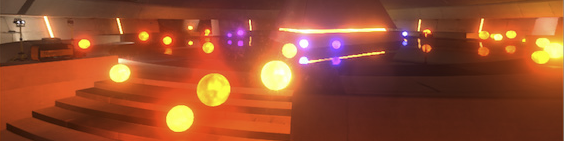
\includegraphics[scale=0.9]{pics/unity-post-processing-bloom}
    \caption{Unity - Post Processing Bloom}
    \label{fig:unity-post-processing-bloom}
\end {figure}
Dieser Effekt kann mithilfe von verschiedenen Parametern angepasst werden.
Die Intensität steuert die Stärke des Effektes, also wie stark das Bild verändert wird.
Der Treshhold filtert alle Pixel, welche unter einem bestimmten Helligkeitsniveau liegen, heraus.
Diese Pixel sind nicht von den Änderungen betroffen.
Wenn Soft Knee auf 1 gestellt wird, ist der Übergang zwischen Pixeln, die durch den Treshhold gefiltert werden, weicher.
Bei 0 befindet sich die Grenze genau auf dem eingestellten Wert.
Der Radius beeinflusst die Ausbreitung des Blooms von einem hellen Objekt aus.
Es kann zusätzlich ein Lens Dirt Effekt angewandt werden, hierbei entstehen Flecken in den hellen Bereichen, siehe Abb. ~\ref{fig:unity-post-processing-lens-dirt}.
~\cite{Unity_Post_Processing_Bloom_2022}

\begin {figure}
    \centering
    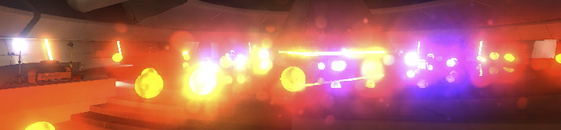
\includegraphics[scale=0.9]{pics/unity-post-processing-lens-dirt}
    \caption{Unity - Post Processing Lens Dirt}
    \label{fig:unity-post-processing-lens-dirt}
\end {figure}

Grain fügt dem angezeigten Bild einen Noise Effekt hinzu.
Hierfür wird ein nahtloses Rauschen angewandt, welches Unvollkommenheiten von Filmbändern ähnelt, siehe Abb. ~\ref{fig:unity-post-processing-grain}.
\begin {figure}
    \centering
    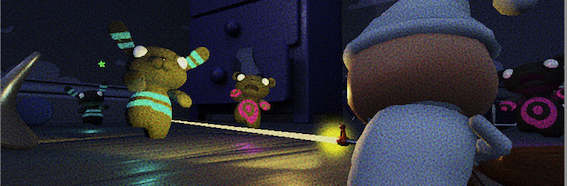
\includegraphics[scale=0.9]{pics/unity-post-processing-grain-on}
    \caption{Unity - Post Processing Grain}
    \label{fig:unity-post-processing-grain}
\end {figure}
Dieser Effekt kann ebenfalls mithilfe von verschiedenen Attributen verändert werden, siehe Abb. ~\ref{fig:unity-post-processing-grain-ui}.
Intensity steuert die Sichtbarkeit des Rauschens im Bild.
Luminance Contribution steuert das Rauschen abhängig von der Helligkeit einer Stelle im Bild.
Bei einem niedrigen Wert ist in dunklen Gebieten kaum Rauschen zu sehen.
Die Größe der Partikel wird vom Size Parameter gesteuert.
\begin {figure}
    \centering
    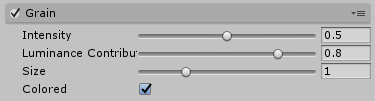
\includegraphics[scale=0.9]{pics/unity-post-processing-grain-ui}
    \caption{Unity - Post Processing Grain UI}
    \label{fig:unity-post-processing-grain-ui}
\end {figure}
~\cite{Unity_Post_Processing_Grain_2022}

Color Grading wird für die Korrektur von Farben und Helligkeit, eines Bildes verwendet.
Ein Beispiel für die Auswirkungen dieses Effekts sieht man in Abbildung ~\ref{fig:unity-post-processing-color-grading-example}.
Der linke Teil des Bildes wurde bearbeitet, der rechte Teil zeigt die ursprünglichen Farben des Bildes an.
Der linke Teil des Bildes wurde bearbeitet, der rechte Teil zeigt die ursprünglichen Farben des Bildes an.
Color Grading hat 5 verschiedene Sektionen, mit welchen genauere Einstellungen getroffen werden können.
Darunter fallen Tonemapping, Basic, Channel Mixer, Trackballs und Grading Curves.
~\cite{Unity_Post_Processing_ColorGrading_2022}
\begin {figure}
    \centering
    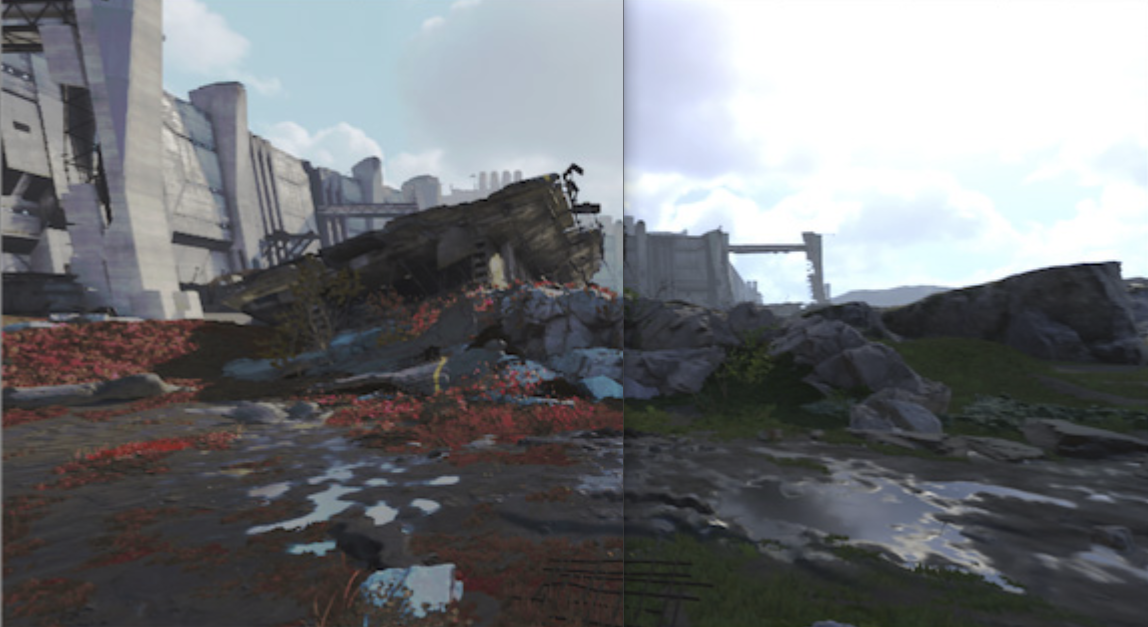
\includegraphics[scale=0.4]{pics/unity-post-processing-color-grading-before-after}
    \caption{Unity - Post Processing Color Grading Example}
    \label{fig:unity-post-processing-color-grading-example}
\end {figure}

Tonemapping beschreibt den Prozess, in welchem HDR Werte eines Bildes so umgewandelt werden, um auf einem Bildschirm dargestellt werden zu können.
Es werden dabei drei Modes zur Verfügung gestellt.
Der Neutral Tonemaper wandelt die Werte, mit möglichst geringem Einfluss auf Farbe und Sättigung, um und verwendet eine Tonemapping Curve, siehe Abb. ~\ref{fig:unity-post-processing-neutral-tonemapper-ui}.
Black In und White In steuern dabei die inneren weißen und schwarzen Kontrolpunkte, Black Out und White Out steuern die äußeren Punkte.
%Mit dem White Level kann auf einen weißen Punkt vor der Kurve eingestellt werden.
White Clip stellt auf einen weißen Punkt nach der Kurve ein.
\begin {figure}
    \centering
    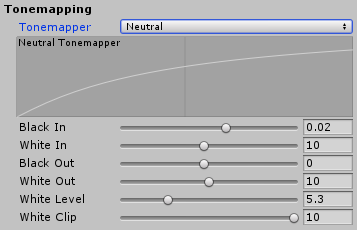
\includegraphics[scale=0.9]{pics/unity-post-processing-color-grading-neutralTonemapper}
    \caption{Unity - Post Processing Neutral Tonemapper UI}
    \label{fig:unity-post-processing-neutral-tonemapper-ui}
\end {figure}

Der Filmic (ACES) Tonemapper verwendet Schätzwerte  des ACES Tonemappers, um ein filmisches Aussehen zu erreichen.
Das Resultat ist ein höherer Kontrast und es wird Einfluss auf die Farbe und Sättigung des Bildes genommen.
Dieser Tonemapper besitzt keine Einstellungsmöglichkeiten, siehe Abb. ~\ref{fig:unity-post-processing-filmic-aces-tonemapper-ui}.

\begin {figure}
    \centering
    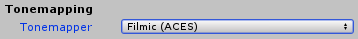
\includegraphics[scale=0.9]{pics/unity-post-processing-color-grading-filmic}
    \caption{Unity - Post Processing Filmic (ACES) Tonemapper UI}
    \label{fig:unity-post-processing-filmic-aces-tonemapper-ui}
\end {figure}

Der Basic Tonemapper stellt simple Einstellungsmöglichkeiten zur Verfügung und ist ein empfohlener Startpunkt für Farbkorrekturen.
Es können Einstellungen wie Post Exposure, Temperature, Tint, Hue Shift, Staturation und Contrast eingestellt werden, siehe Abb. ~\ref{fig:unity-post-processing-basic-tonemapper-ui}.
\begin {figure}
    \centering
    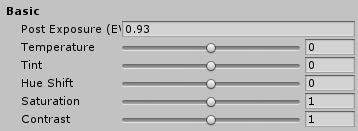
\includegraphics[scale=0.9]{pics/unity-post-processing-color-grading-basicTonemapper}
    \caption{Unity - Post Processing Basic Tonemapper UI}
    \label{fig:unity-post-processing-basic-tonemapper-ui}
\end {figure}

Post Exposure stellt die allgemeine Belichtung der Scene in EV Einheiten dar.
Dieser Effekt wird erst nach den HDR Effekten, aber vor dem Tonemapping, eingesetzt, damit die vorherigen Effekte nicht beeinflusst werden.
Die Temperatur setzt die White Balance zu einer beliebig eingestellten Farbtemperatur.
Mithilfe von Tint kann ein grüner oder magenta Tint im Bild korrigiert werden.
Hue Shift verschiebt das HUE aller Farben, während Saturation die Intensität dieser beeinflusst.
Der Contrast erweitert oder verkleinert die Breite zwischen den dargestellten Farben.

Mithilfe des Channel Mixers kann der Einfluss der einzelnen Farbkanäle, welche Rot, Grün und Blau sind, auf das gesamte Bild eingestellt werden.
Wie in Abb. ~\ref{fig:unity-post-processing-channel-mixer-ui} zu sehen ist, kann dabei jeder Farbkanal einzeln mittels eines Schiebereglers verändert werden.
Ein Beispiel für die Auswirkungen dieses Effekts ist in Abb. ~\ref{fig:unity-post-processing-channel-mixer} zu erkennen.
\begin {figure}
    \centering
    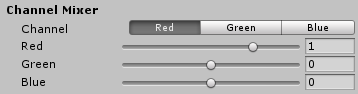
\includegraphics[scale=0.9]{pics/unity-post-processing-channel-mixer-ui}
    \caption{Unity - Post Processing Channel Mixer UI}
    \label{fig:unity-post-processing-channel-mixer-ui}
\end {figure}

\begin {figure}
    \centering
    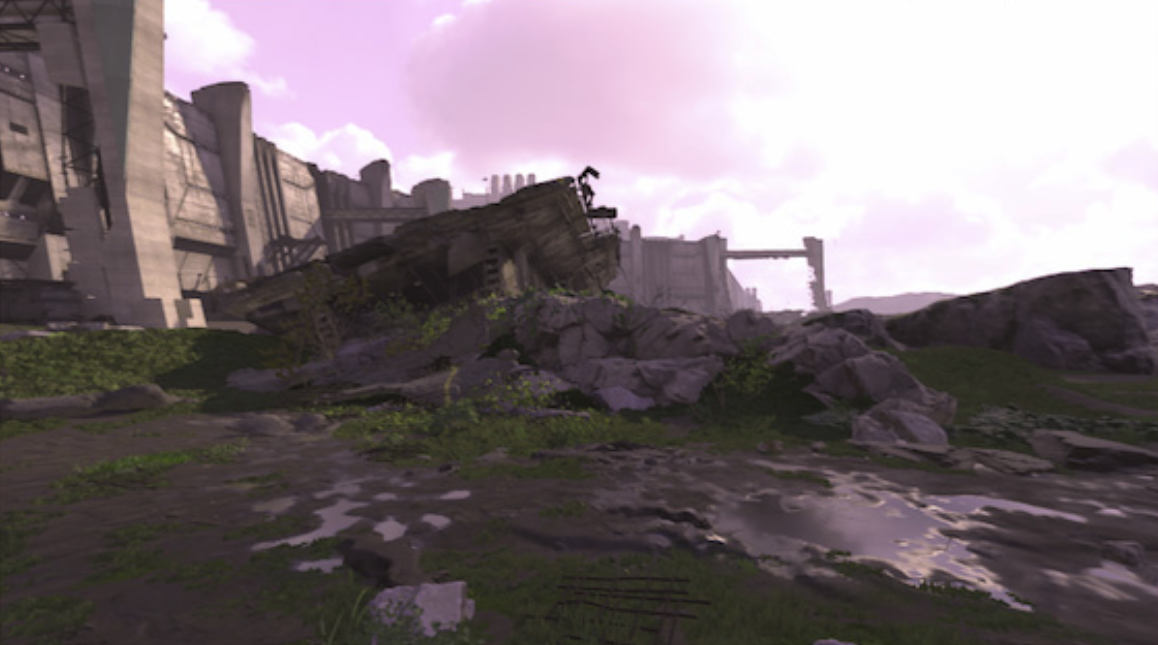
\includegraphics[scale=0.4]{pics/unity-post-processing-channel-mixer-example}
    \caption{Unity - Post Processing Channel Mixer}
    \label{fig:unity-post-processing-channel-mixer}
\end {figure}

Mithilfe von Trackballs kann man ein 3-Wege Color Grading in einem Linearen oder Logarithmischen System vornehmen.
Bei der Logarithmus Variante werden die Farbverteilung und der Contrast komprimiert um einen Color-Timing Process, welcher von optischen Film Druckern erzeugt wird, zu simulieren, siehe Abb. ~\ref{fig:unity-post-processing-trackballs-log}.
Hierbei kann mit Power das Gamma und mit Offset das Signal beeinflusst werden.
\begin {figure}
    \centering
    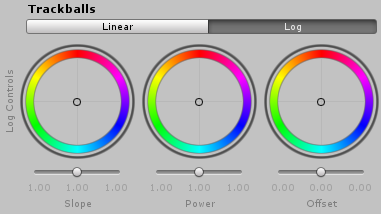
\includegraphics[scale=0.9]{pics/unity-post-processing-trackballs-log}
    \caption{Unity - Post Processing Trackballs Log}
    \label{fig:unity-post-processing-trackballs-log}
\end {figure}
Die Lineare Methode wurde für linear-encododed Data optimiert, siehe Abb. ~\ref{fig:unity-post-processing-trackballs-linear} für das UI.
Mithilfe von Lift kann das gesamte Signal verschoben werden.
Gamma beeinflusst wieder die mittleren Töne und Gain verstärkt das Signal.
\begin {figure}
    \centering
    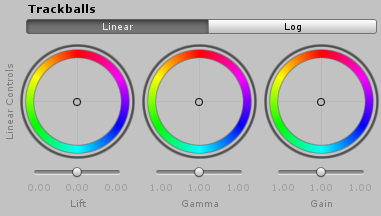
\includegraphics[scale=0.9]{pics/unity-post-processing-trackballs-linear}
    \caption{Unity - Post Processing Trackballs Linear}
    \label{fig:unity-post-processing-trackballs-linear}
\end {figure}

Mithilfe von fünf verschiedenen Grading Curves können YRGB, Hue vs Hue, Hue vs Sat, Sat vs Sat und Lum vs Sat verändert werden.
Hierbei handelt es sich jedesmal um eine Kurvendarstellung, in welcher man weitere Punkte setzen und damit den Verlauf der Kurve beeinflussen kann, siehe Abb. ~\ref{fig:unity-post-processing-grading-curve-example}.
\begin {figure}
    \centering
    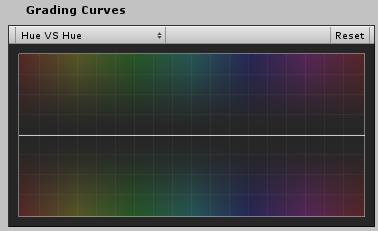
\includegraphics[scale=0.9]{pics/unity-post-processing-grading-curve-example}
    \caption{Unity - Post Processing Grading Curve Example}
    \label{fig:unity-post-processing-grading-curve-example}
\end {figure}
Bei der YRGB Kurve kann durch die Manipulation des Graphen der Contrast und die Helligkeit des Bildes eingestellt werden.
Die Hue vs Hue Kurve bietet die Möglichkeit, Farbbereiche zu verfeinern oder auszutauschen.
Um eine bestimmte Farbe besonders hervorzuheben oder einen monochromatischen Effekt zu erreichen, wird die Hue vs Sat Kurve verwendet.
Bei der Sat vs Sat Kurve werden einfache Veränderungen der Farbe wie beim Color Grading vorgenommen.
Die letzte Option heißt Lum vs Sat Kurve und ermöglicht es, in bestimmten Gebieten die Sättigung zu verringern, wie zum Beispiel in dunklen Stellen.

\subsection{Nebel}\label{subsec:fog-effect}
\setauthor{Florian Beckerle}
Unity bietet mehrere M\"oglichkeiten, Nebel darzustellen, zum Beispiel mittels Post Processing, oder mithilfe der Lighting Einstellungen.
F\"ur BeamVR wurde die zweite Variante verwendet, da der Nebel in BeamVR kein Hauptaugenmerk ist und mithilfe dieser Methode das Einstellen für BeamVR schneller ging.
~\cite{Unity_Lighting_Window_2022}

Mittels Post Processing wird ein Screen-Space Nebel Effekt in der Tiefen-Texture der Kamera erstellt, siehe Abb. ~\ref{fig:unity_post_processing_fog}.
Screen-Space bedeutet, dass die Position auf dem Bildschirm und nicht in der dreidimensionalen Welt berechnet wird.
~\cite{Unity_Fog_2022}

\begin {figure}
    \centering
    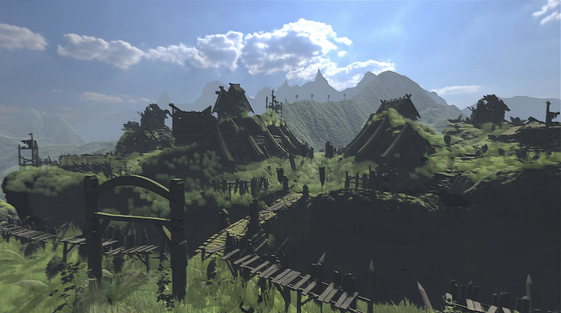
\includegraphics[scale=0.9]{pics/unity-post-processing-fog}
    \caption{Unity - Post Processing Fog}
    \label{fig:unity_post_processing_fog}
\end {figure}
Unter dem Begriff Map versteht man eine Umgebung in einer Spielwelt, in diesem Fall wird auf die Szenen, in welchen die Städte platziert sind, verwiesen.
Auf fast jeder Map von BeamVR wurde dieser Nebel verwendet.
In der Nacht Map wird mithilfe dieses Effekts ein leichter Nebel dargestellt, was zur abendlichen Stimmung beitr\"agt.
Bei Apocalypse ist der Nebel viel dichter und stellt einen Sandsturm dar. Zus\"atzlich wurde dieser gelb gef\"arbt, um noch mehr an Sand zu erinnern, siehe Abb. ~\ref{fig:beamvr_yellow_fog}.

\begin {figure}
    \centering
    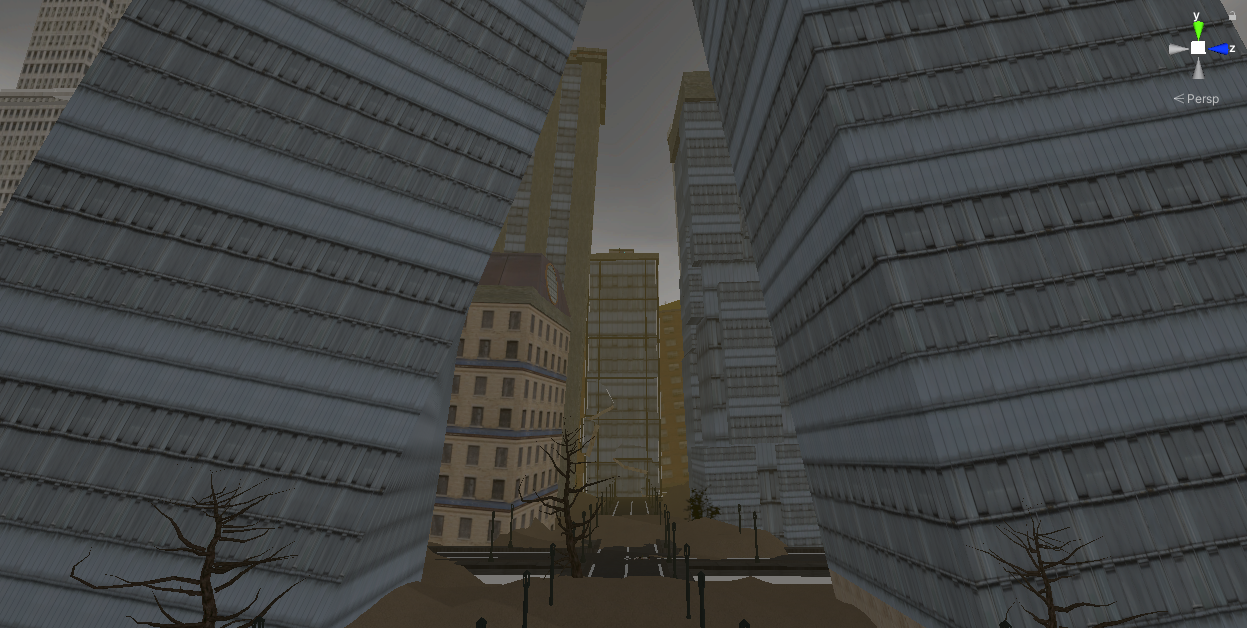
\includegraphics[scale=0.3]{pics/beamvr_yellow_fog}
    \caption{Beam VR - Yellow Fog}
    \label{fig:beamvr_yellow_fog}
\end {figure}

Mittels der High Definition Render Pipeline, welche auch als HDRP bezeichnet wird, kann ebenfalls Nebel eingestellt werden.
Hierfür wird die Volume Framework benötigt, in welcher ein Nebel Overrride hinzugefügt wird.

Diese Framework bietet einige verschiedene Optionen zur Beeinflussung des Nebels, siehe Abb. ~\ref{fig:unity-hdrp-fog}.
Die Option Enable wird verwendet, um den Effekt zu aktivieren oder deaktivieren.
Die Fog Attenuation Distance bestimmt die Dichte und die Sichtweite im Nebel.
Ab der eingestellten Distanz hat der Nebel bereits 63\% des Umgebungslichts absorbiert.
Dichte und Sichtweite bleiben bis zu einer definierten Base Height constant, erst ab dieser ist eine exponentielle Abnahme beider Attribute erkennbar.
Die Maximum Height und Max Fog Distance bestimmen die Stärke des Abfalls und die Distanz des Nebels.
Mittels des Color Modes kann die Farbe des Nebels beeinflusst werden.
Bei Sky Color wird die Farbe automatisch an den Himmel angepasst, während bei constant Color eine eigene Farbe eingestellt werden kann.

Volumetric Fog kann mittels der gleichnamigen Option aktiviert werden.
Die Albedo Option setzt dabei die Farbe des Nebels, mit welcher das Licht gestreut wird.
Lichter werden, mit zunehmender Dichte des Nebels, schneller abgedunkelt.
Anisotropy steuert die Streuung des Lichtes.
0 streut das Licht gar nicht, 1 streut das Licht vorwärts und -1 streut rückwärts.
Mittels eines Filters kann eine Unschärfe der eingehenden Lichter geschaffen werden, damit ein weicherer Übergang zustande kommt.
~\cite{Unity_HDRP_Fog_2022}

\begin {figure}
    \centering
    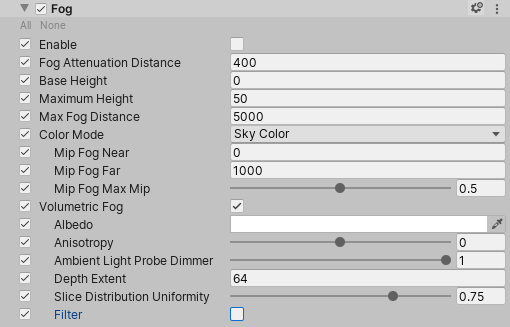
\includegraphics[scale=0.9]{pics/unity-hdrp-fog}
    \caption{Unity - HDRP Fog}
    \label{fig:unity-hdrp-fog}
\end {figure}


\subsection{Lichter}\label{subsec:light-effect}
\setauthor{Florian Beckerle}
In der Nacht Map wurden die von Unity bereitgestellten Point-Lights als Straßenlichter benutzt.
Point Lights k\"onnen mithilfe eines Radius auf einen bestimmten kreisf\"ormigen Bereich eingegrenzt werden.
Weiters wird mithilfe der Lichtst\"arke die Wirkkraft des Lichtes in diesem Gebiet genauer bestimmt.
Dank dieser Eigenschaften war das Point Light f\"ur die Aufhellung der Straßen, siehe Abb. ~\ref{fig:beamvr_street_lights}.
~\cite{Unity_PointLights_2022}
\begin {figure}
    \centering
    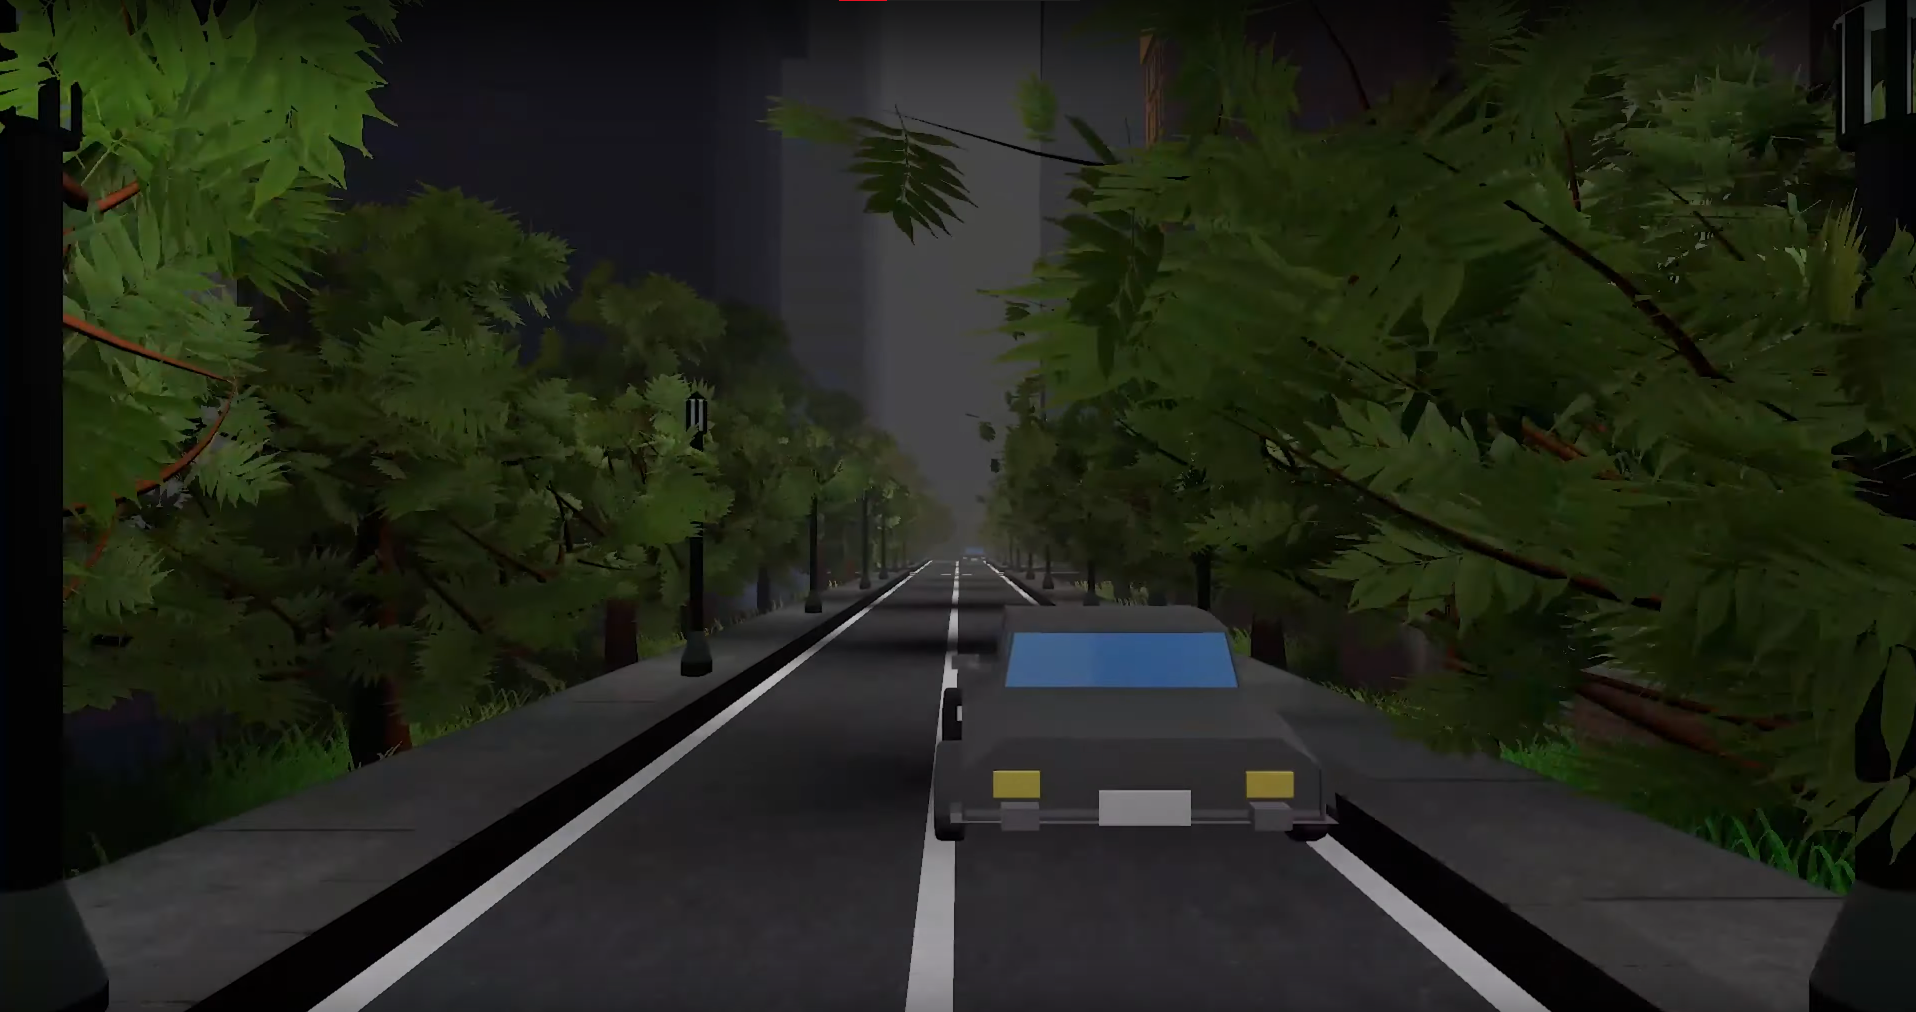
\includegraphics[scale=0.3]{pics/beamvr_point_lights}
    \caption{Beam VR - Street Lights}
    \label{fig:beamvr_street_lights}
\end {figure}

\subsection{Wind}\label{subsec:wind-effect}
Damit sich die B\"aume und B\"usche in BeamVR wie im Wind bewegen, werden Unitys Wind Zones ben\"otigt.
Diese Zonen sind bestimmte Bereiche, in welchen eine Windrichtung, Windst\"arke und Turbulenz definiert wird.
Die eingestellten Effekte werden dann auf alle Objekte angewandt, die mithilfe des Terrains oder Particle Systems iniziiert wurden.
~\cite{Unity_WindZones_2022}

\section{Unity Prefabs}
\label{sec:prefabs}
\setauthor{Quirin Ecker}

In Unity gibt es ein System welches dem Entwickler oder der Entwicklerin erlaubt eine bestimmte Zusammenstellung von 3d Elementen zu speichern und mehrmals in verschiedenen Szenen zu verwenden.
Diese Zusammenstellungen von 3d Elementen heißen auch Prefabs.
Wird dieses Prefab verändert, wird es an jeder platzierten Stelle aktualisiert.
Es werden dabei die Komponenten und Positionen der einzelnen Elemente relativ zu dem Prefab gespeichert.

Prefabs können auch überschrieben werden an der Stelle wo sie platziert worden sind.
Aus Erfahrung zeigt sich aber, dass dies mit Vorsicht zu genießen ist, da lokale Änderungen nicht mehr global überschrieben werden.
Somit haben globale Änderungen keinen wirklichen Einfluss auf das lokale Prefab.
Außerdem können Prefabs auch ineinander verschachtelt werden~\cite{Unity_Prefabs}.

In der BeamVR Applikation wird dieses System an mehreren Stellen verwendet.
Diese Prefabs wurden beispielsweise in der BeamVR Applikation für einzelne Elemente, welche in allen Karten existieren, benutzt.
Alle diese Elemente werden in ein sogenanntes Game Prefab gruppiert, welches in allen Karten platziert wird.

Folgend werden das Game Prefab und zwei weitere für BeamVR relevante Prefabs noch genauer beschrieben.

\subsection{Game}\label{subsec:game-prefab}

Wie bereits beschrieben befinden sich alle Game relevant Elemente in dem Game Prefab.
Somit wird dieses Prefab in allen Karten Szenen verwendet.
Nur in der Menü- und Setup-Szenen wird dieses Prefab nicht gebraucht.

Folgend sind die wichtigsten Elemente des Game Prefab aufgelistet:

\begin{itemize}
    \item \textbf{Beam:} Der Beam ist der virtuelle Balken, der von dem Hochhaus absteht.
    \item \textbf{Collider:} Die Collider sind Elemente, welche Aktionen auslösen, wenn ein anderes Element mit diesen kollidiert.
    Visuelle sind diese Collider unsichtbar.
    \item \textbf{GameCameraRig:} Das~\emph{GameCameraRig} ist ein weiteres Prefab, welches für VR spezifische Elemente zuständig ist.
\end{itemize}


\subsection{GameCameraRig}\label{subsec:game-camera-rig}

Wie bereits im Game Prefab beschrieben ist das GameCameraRig Prefab ein bestandteil des Game Prefab und beinhaltet alle VR spezifischen Elemente.
Dieses Prefab ist ein abgeändertes CameraRig Prefab, welches bereits von dem SteamVR Plugin zur Verfügung gestellt worden ist.
Das Prefab an sich soll den VR Raum darstellen.

Folgende sind die wichtigsten Elemente des GameCameraRig Prefab aufgelistet:

\begin{itemize}
    \item \textbf{Controller:} Die Controller sind Elemente welche eine SteamVR Controller Script-Component beinhalten.
    Durch dieses Script befindet sich dieses Element in der richtigen Position und Orientierung relativ zu der VR Fläche.
    \item \textbf{Camera:} Genauso wie die Controller Elemente besitzt das Camera Element auch ein Script.
    Mit diesem Script nimmt die Kamera die Position und Orientierung des Headsets relativ zur VR Fläche an.
    Diese Kamera ist auch für die Sicht des Spielers zuständig.
    \item \textbf{Tracker Objekte} Diese Elemente haben ebenfalls wieder ein ähnliches Script.
    Durch dieses Script befindet sich dieses Element in der gleichen Position und Orientierung des physischen Tracker.
    In der Script Komponente kann in einem Auswahlmenü der richtige Tracker eingestellt werden.
    \item \textbf{Spieler Modell:} Das Spieler Modell ist das Modell, welches nach dem Kalibrieren des Full-Body-Trackings die Pose des Spielers einnimmt.
    \item \textbf{VRIK Calibration Controller:} Bei diesem Element befindet sich ein Script-Component, in dem das Full-Body-Tracking konfiguriert werden kann.
    Für mehr Informationen wird auf Abschnitt~\ref{sec:final-ik-plugin} verwiesen.
\end{itemize}

\subsection{MenuCameraRig}\label{subsec:menu-camera-rig}

Das MenuCameraRig ist genauso wie das GameCameraRig eine Abänderung des von SteamVR Plugin bereitgestellte CameraRig.
Im Gegensatz zum GameCameraRig wird das MenuCameraRig nicht in den 3 Karten verwendet.
Das MenuCameraRig wird in den Menü-Szenen verwendet und besteht aus Menü und VR spezifische Elemente.

Viele Elemente sind gleich wie bei dem GameCameraRig.
Der große Unterschied des MenuCameraRig ist, dass die Controller noch weitere Script-Componenten beinhalten.
Diese sind Input Scripts welche für den Auswahlstrahl und das Auswählen der Menü-Elemente verantwortlich sind.

%TODO: (Quirin Ecker)(optional) Möglichkeit für ein Bild eines Inputstrahls

Weiters sind viele der game-spezifischen Elemente in diesem Prefab nicht vorhanden.
Beispielsweise gibt es keine Full-Body-Tracking Elemente, wie das Spieler-Modell und der VRIK-Calibration-Controller.


\begin{spacing}{1}
\chapter{Zusammenfassung}
\end{spacing}
Mit BeamVR wurde eine einfache Augmented Virtuality Applikation entwickelt.
Hiermit wurde gezeigt, dass reale Elemente in einer virtuellen welt die Immersion und den realismus stark verstärken.

Durch einen einfachen Balken, welcher sich für gewöhnlich nicht bewegt, wurde eine Augmented Virtuality Applikation entwickelt.
Mit zusätzlichen Funktionalitäten, wie dem Full Body Tracking und einer vielfältigen Umgebung wird gezeigt, dass es mit dieser Kombination möglich ist eine starke Immersion zu erzeugen.

Um eine Applikation wie diese in Betrieb zu nehmen, sind viele Schritte involviert.
Dabei versucht unsere Applikation die Konfigurationen und Schritte zu minimieren.
Beispielsweise benützen wie möglichst viele Informationen von SteamVR.

Für einen gewissen Spannungsaufbau kann die Benutzerin oder der Benutzer auch von dem Balken herunterfallen.
Fällt die Benutzerin oder der Benutzer von dem Balken, fällt dieser ebenso von dem Hochhaus in der Applikation herunter.

Durch viele Einflussfaktoren bei dem Setup der Applikation, kommt es teilweise zu unerwarteten Resultaten.

Beispielsweise kommt es oft zu Drehungen des VR Raumes in der virtuellen Realität.
Durch die Drehung muss der VR Raum neu kalibriert werden oder die physische Anordnung abgeändert werden, da der Balken beispielsweise in die falsche Richtung schaut.
Dies kann bei Veranstaltungen zu minimalen Problemen führen.

Außerdem ist die Stabilität der Software noch nicht auf dem erhofften Stand.
Dadurch können plötzliche Probleme bei dem Full-Body-Tracking und der Balken Kalibrierung auftauchen.

Zukünftig soll die Stabilität der Software noch verbessert werden, damit die Applikation mit einer niedrigeren Fehlerwahrscheinlichkeit präsentierbar ist.

Außerdem würde eine Auswahl von Charakteren und weiteren Karten mehr Abwechslung in die Applikation bringen.

In dem Augmented Virtuality Spektrum besteht noch sehr viel Potenzial.
Dabei besteht die Möglichkeit noch mehr Elemente in die virtuelle Realität einzubauen und damit neue Prinzipien zu entwickeln.

Für nachfolgende Diplomarbeiten könnte, zum Beispiel ein anderes Szenario, gewählt werden.
Hierbei besteht bereits die Idee für einen Balken, welcher an der Spitze eines Zuges angebracht ist.


\newpage
\pagenumbering{Roman}
\setcounter{page}{\value{RPages}}
\newacronym{guid}{GUID}{Globally Unique Identifier}
\newacronym{jit}{JIT}{Just In Time Compiler}
\newacronym{nfc}{NFC}{Near Field Communication}
\newacronym{rfid}{RFID}{Radio Frequency Identification}

% Usage:
% \gls{label} lowercase in text
% \Gls{label} Uppercase in text
% \newacronym{label}{abbrev}{full}
% \newglossaryentry{label}{settings}



%\setlength{\glsdescwidth}{0.8\linewidth}
\glsnogroupskiptrue
\printglossary[title=Glossar,toctitle=Glossar] %,style=long]
\spacing{1}{
%\bibliographystyle{IEEEtran}
\bibliographystyle{ieeetrande}
\bibliography{bib}
}
\listoffigures
\listoftables
\lstlistoflistings
\appendix
\addchap{Anhang}
\input{./sections/appendix}
\end{document}

